\begin{savequote}[8cm]
\textlatin{Neque porro quisquam est qui dolorem ipsum quia dolor sit amet, consectetur, adipisci velit...}

There is no one who loves pain itself, who seeks after it and wants to have it, simply because it is pain...
  \qauthor{--- Cicero's \textit{de Finibus Bonorum et Malorum}}
\end{savequote}

\chapter{\label{ch:tuning}TKI Tuning}

\minitoc

Current neutrino interaction models are effective models, i.e. they have variable parameters, aiming to parameterize our ignorance of the true underlying physics.
These parameters can be constrained by comparing model predictions to data, which is the so-called tuning process.
The data used in tuning are the cross section measurements from various neutrino experiments.
A successfully tuned model will have a better agreement with the data used in tuning than the original model, and it could also shed light on the direction of future model development.
The validity of the tuned model can be tested against new data.
In view of the incoming data collected by the upgraded ND280, it is the perfect time to tune the current model to the existing data to maximize the utility of the new data.
The GENIE collabration has developed a comprehensive tuning framework, and has collected an extensive database of neutrino, charged lepton, and hadron scattering measurements. 
Hence, we have performed the tuning of an effective model in \genie using this frameowrk.
The procedures and the results are presented in this chapter~\footnote{This chapter is based on the work published in Ref.~\cite{GENIE:2024ufm}.}.

\section{\label{sec:Tuning}Tuning procedure}
This study employs the tuning procedure delineated in Ref.~\cite{GENIE:2022qrc}, utilizing $N_{\textrm{par}}$ model parameters. 
The primary objective is to determine the best fit—that is, the optimal set of parameter values—within the parameter space by minimizing the $\chi^2$ between the model predictions and the experimental data. 
Due to the high dimensionality of the parameter space, a brute-force, grid-based point-by-point scan is impractical. 
Therefore, a sufficiently large number of points in the model parameter space is sampled at random, with each point initiliating a full simulation. 
Subsequently, the simulation output for each data observable bin is parametrized using Professor~\cite{Buckley:2009bj} with a polynomial of the model parameters of a given order, $N_{\textrm{ord}}$. 
The minimal number of points ($N_{\textrm{s}}$) required for tuning $N_{\textrm{par}}$ parameters with a polynomial of order $N_{\textrm{ord}}$ is determined by the combinatorial formula,
\begin{equation}
    N_{\textrm{s}} = \binom{N_{\textrm{par}}+N_{\textrm{ord}}}{N_{\textrm{ord}}}.
\end{equation}
Since $N_\textrm{s}$ increases factorially, it is imperative to exercise caution when increasing either the number of parameters or the polynomial degree. 
Given that our tuning incorporates all $2$ \sfcfg\ and $12$ hA parameters (see Sec.~\ref{sec:tuning-para-choice}), a fourth-order parameterization necessitates over 6,000 simulation generations, which are already computationaly expensive.
Thus, only polynomials up to order $4$ are considered, a choice that has been shown to reproduce the MC predictions satisfactorily, as illustrated in Fig.~\ref{fig:residual}. 
\begin{figure}[!htb] 	
    \centering 		
    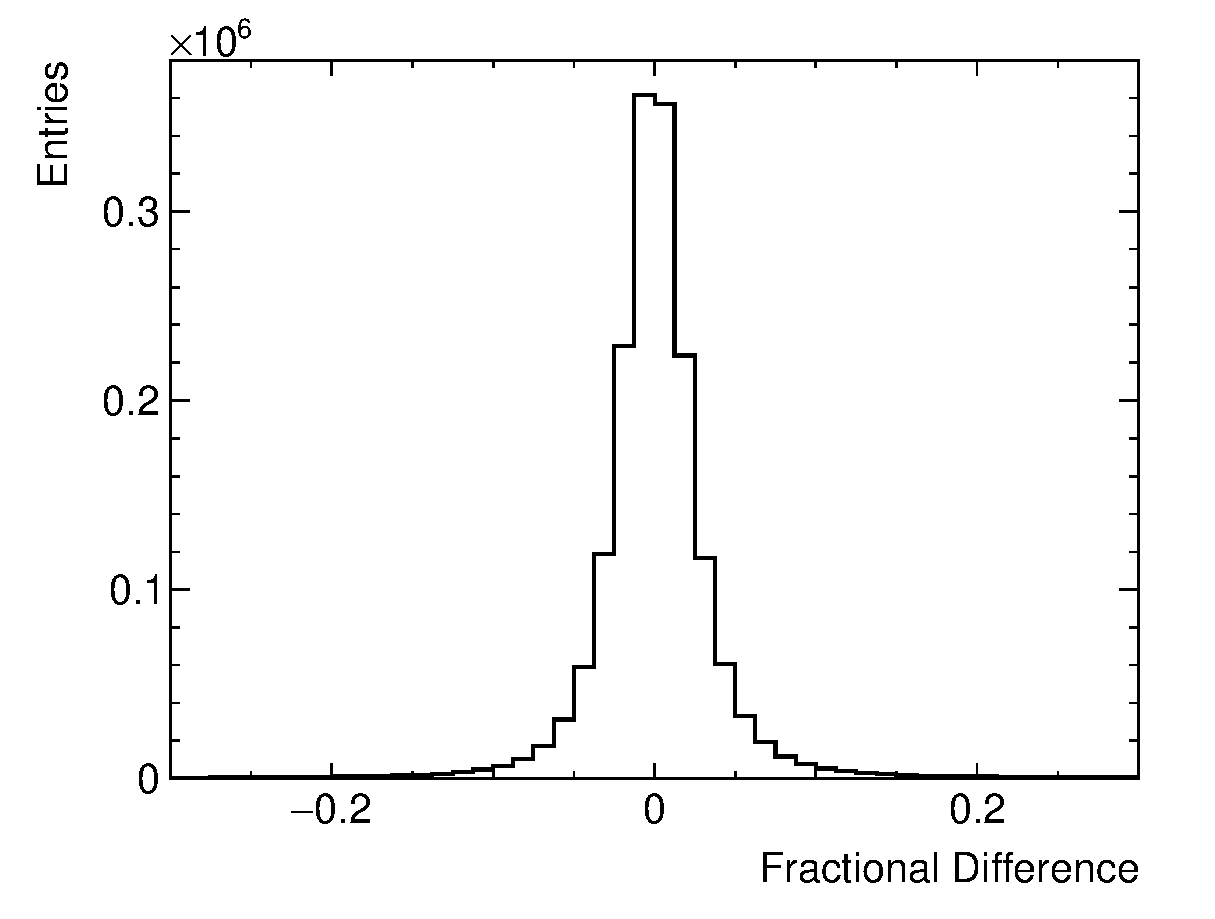
\includegraphics[width=\sgfigwid\textwidth]{figures/tuning/residual.eps}
    \caption{\label{fig:residual} Fractional difference for the bin-by-bin cross sections between MC truth and the parameterized approximation using fourth-order polynomials, both in the Norm-Shape (NS)~\cite{DAgostini:1993arp,Hanson:2005mrg} space with \allpar. See Table~\ref{tab:hALFG-para} for the definition of \allpar. The residual exhibits a mean of $0.003$ and a standard deviation of $0.073$.} 
\end{figure}

Furthermore, to circumvent Peelle's Pertinent Puzzle~\cite{PPP_FNL,Chakrani:2023htw}~\footnote{This is a phenomenon where unknown correlations between observables can skew the $\chi^2$ minimizaion.}, the Norm-Shape (NS) transformation prescription~\cite{DAgostini:1993arp,Hanson:2005mrg} is adopted. 
Thereafter, the extremal point is determined by minimizing $\chi^2$ between the NS-transformed polynomial approximation and the NS-transformed data. 
During the minimization process, priors—typically derived from systematic uncertainties—are imposed on each parameter to prevent them from deviating excessively from their nominal values. 
The following subsections elaborate on the specific measurement observables and model parameters to be tuned.

\section{Inputs}
The first step towards tuning is to identify the models to be tuned and the data to be used by spotting the lacking area of the current model, which is manifested by the data-MC discrepancy.
One such example is illustrated in Fig.~\ref{fig:g24-0-dat-reac} and Fig.~\ref{fig:g24-0-pn-reac}, which shows the data-MC comparison using \newtune\, one of the latest Comprehensive Model Configurations (CMC) in \genie, for four TKI measurements, namely \ttkzpi~\cite{T2K:2018rnz}, \ttkpip~\cite{T2K:2021naz}, \minzpi~\cite{MINERvA:2018hba, MINERvA:2019ope}, and \minpiz~\cite{MINERvA:2020anu}. 
\begin{figure*} 
    \centering 		
    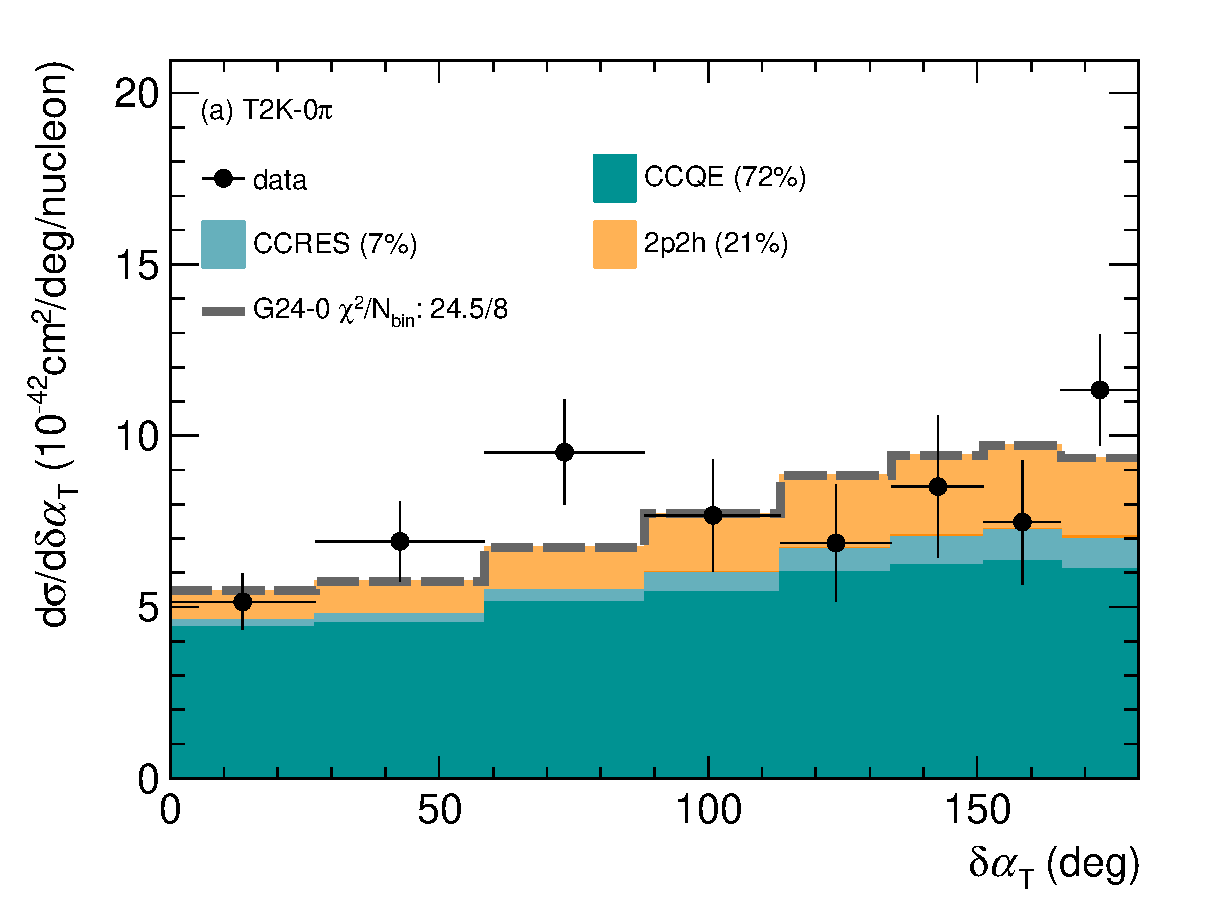
\includegraphics[width=\dbfigwid\textwidth]{figures/tuning/0000-t2k_0pi_dalphat_reac_decomp.eps} 
    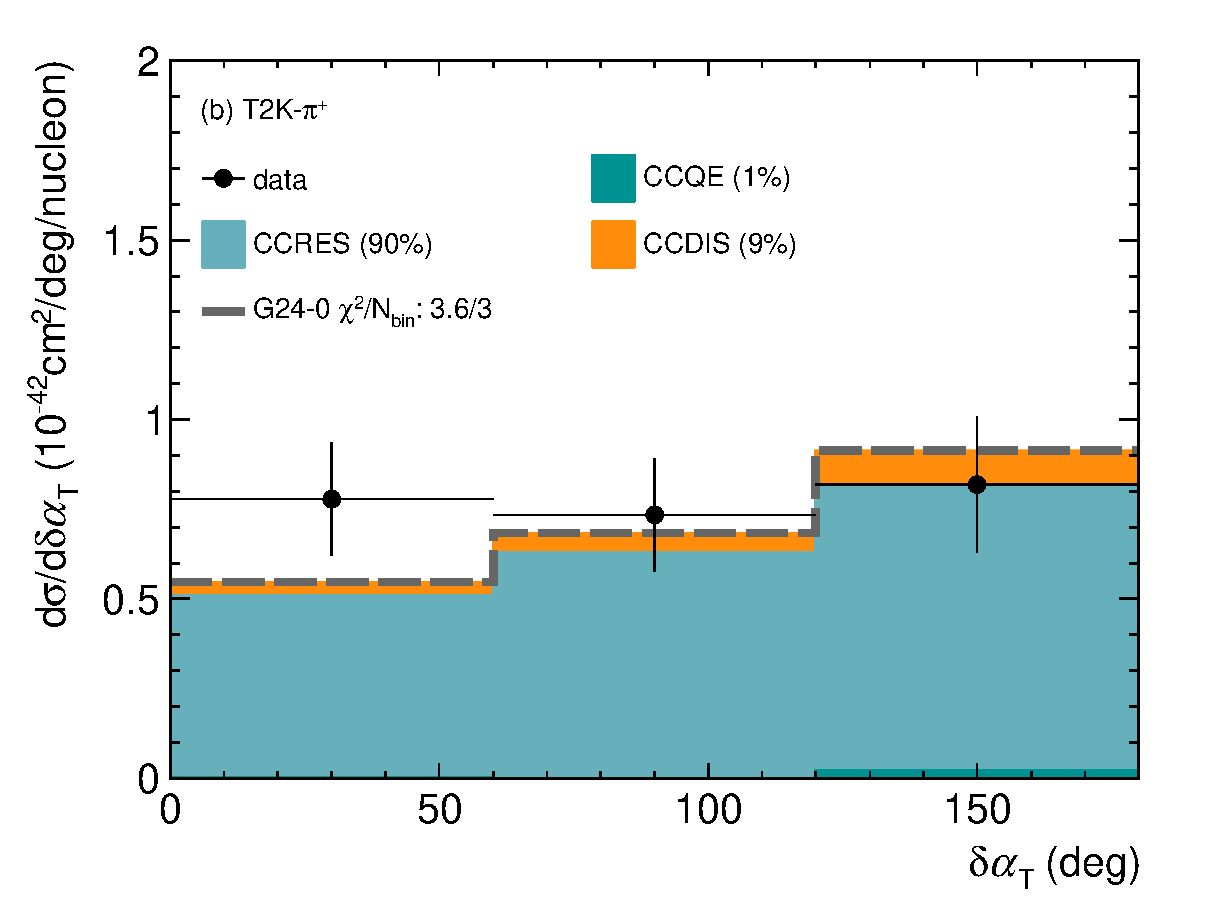
\includegraphics[width=\dbfigwid\textwidth]{figures/tuning/0000-t2k_pip_dalphat_reac_decomp.eps} 
    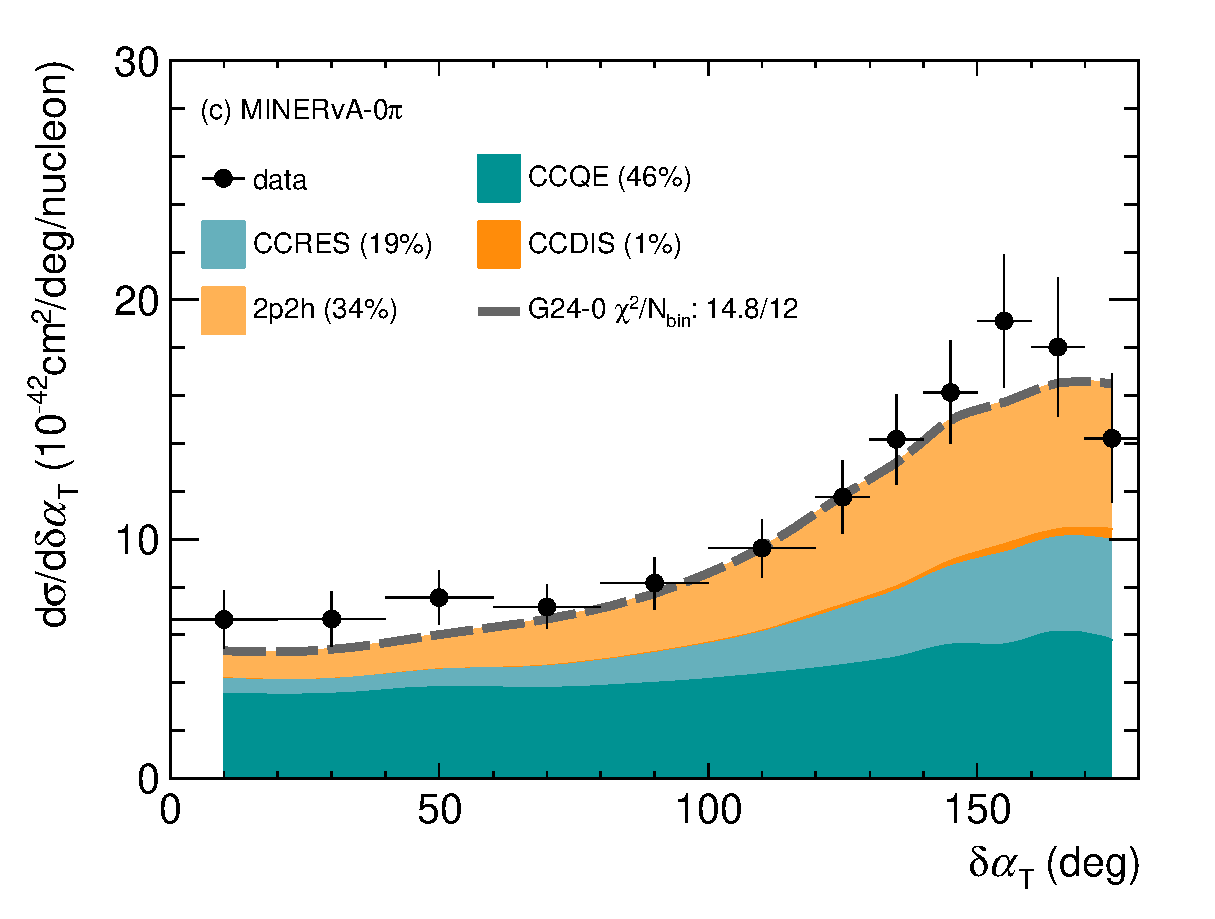
\includegraphics[width=\dbfigwid\textwidth]{figures/tuning/0000-min_0pi_dalphat_reac_decomp.eps} 
    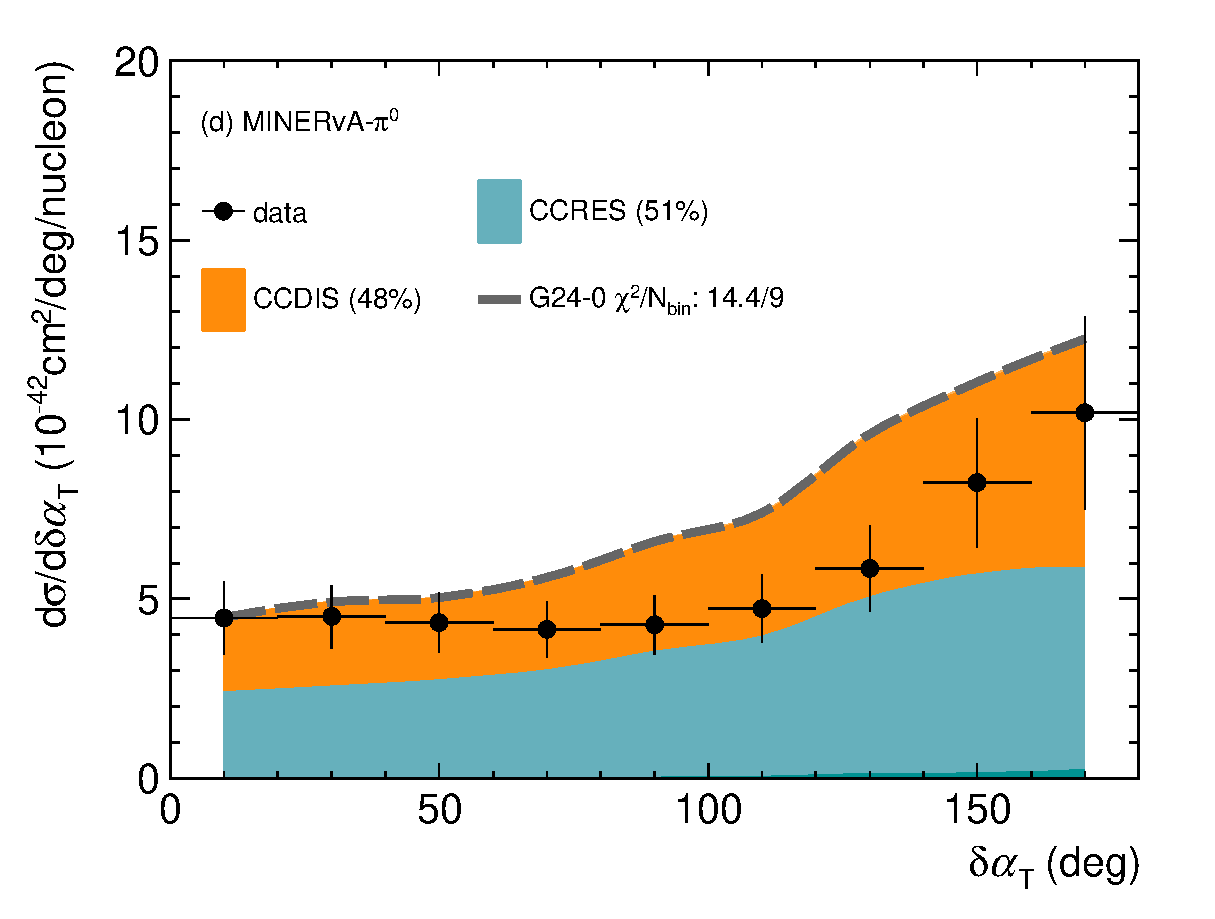
\includegraphics[width=\dbfigwid\textwidth]{figures/tuning/0000-min_pi0_dalphat_reac_decomp.eps}
    \caption{$\dat$ measurements decomposed in interaction types, compared to \gZero prediction.}   \label{fig:g24-0-dat-reac} 
            
    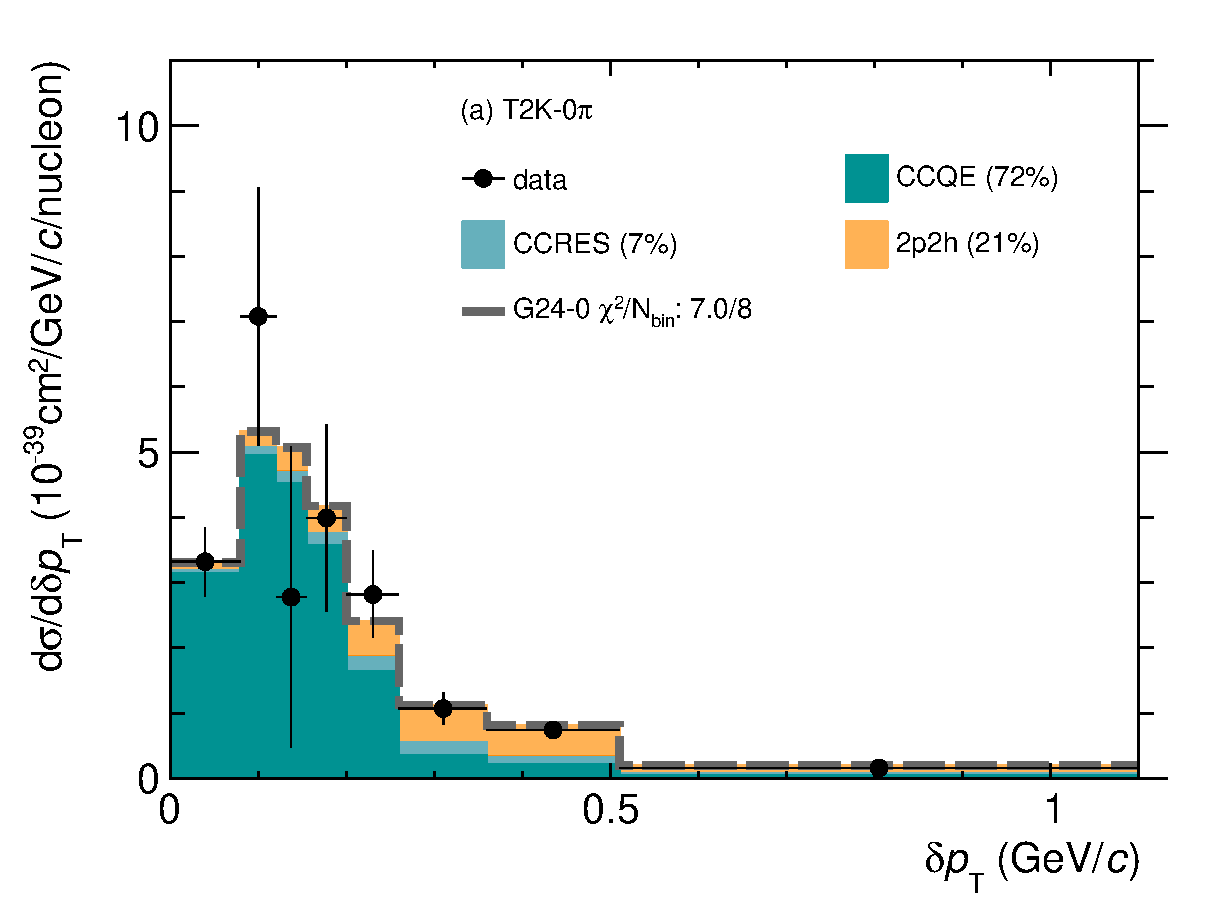
\includegraphics[width=\dbfigwid\textwidth]{figures/tuning/0000-t2k_0pi_dpt_reac_decomp.eps}
    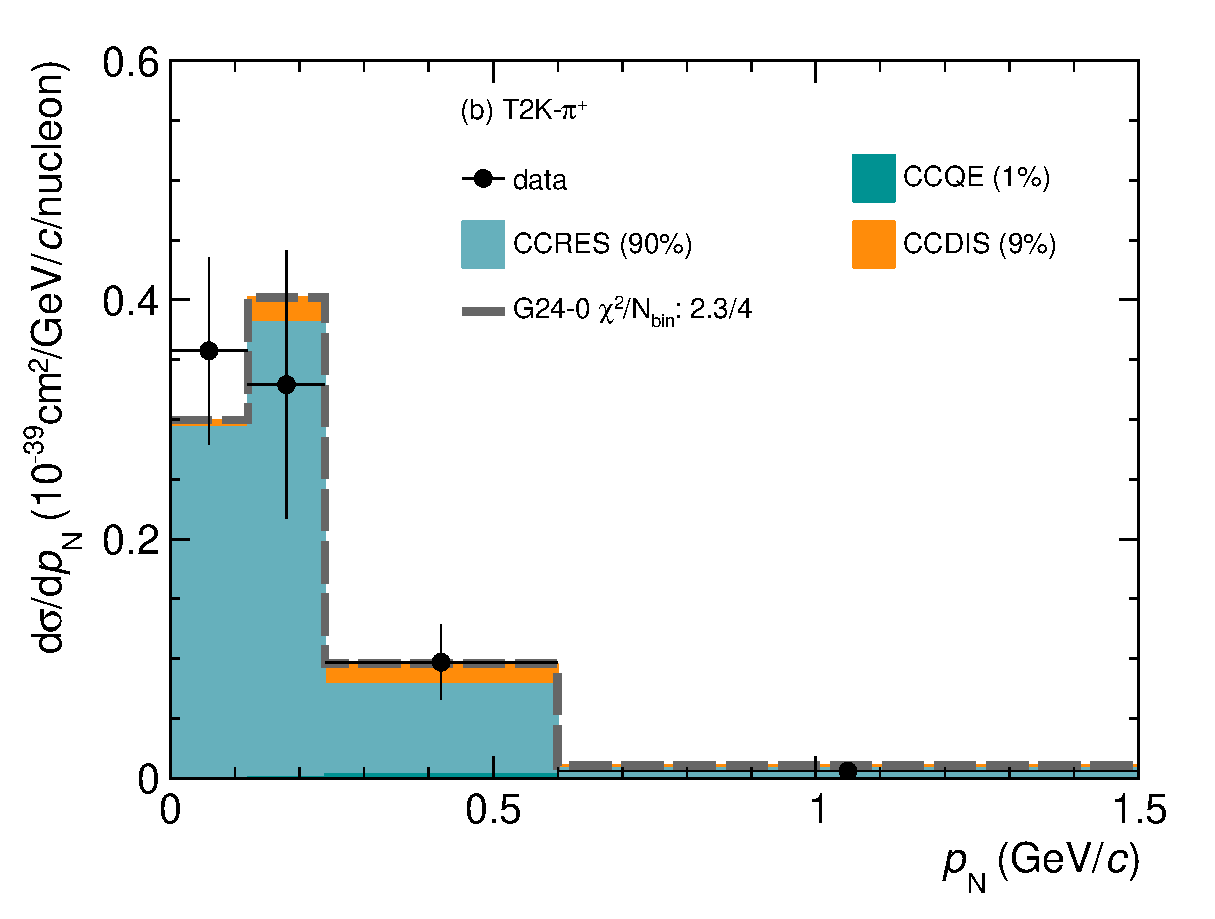
\includegraphics[width=\dbfigwid\textwidth]{figures/tuning/0000-t2k_pip_pn_reac_decomp.eps}
    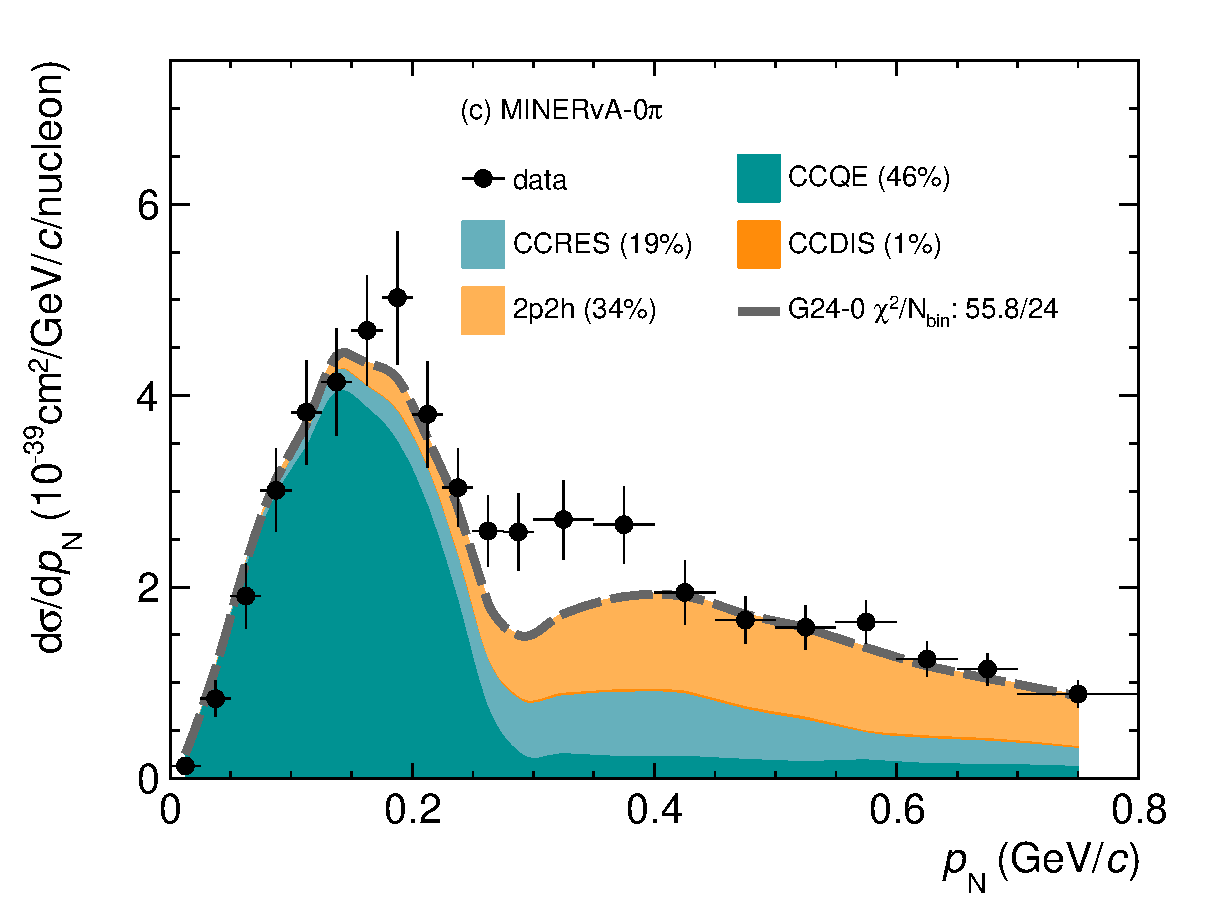
\includegraphics[width=\dbfigwid\textwidth]{figures/tuning/0000-min_0pi_pn_reac_decomp.eps}
    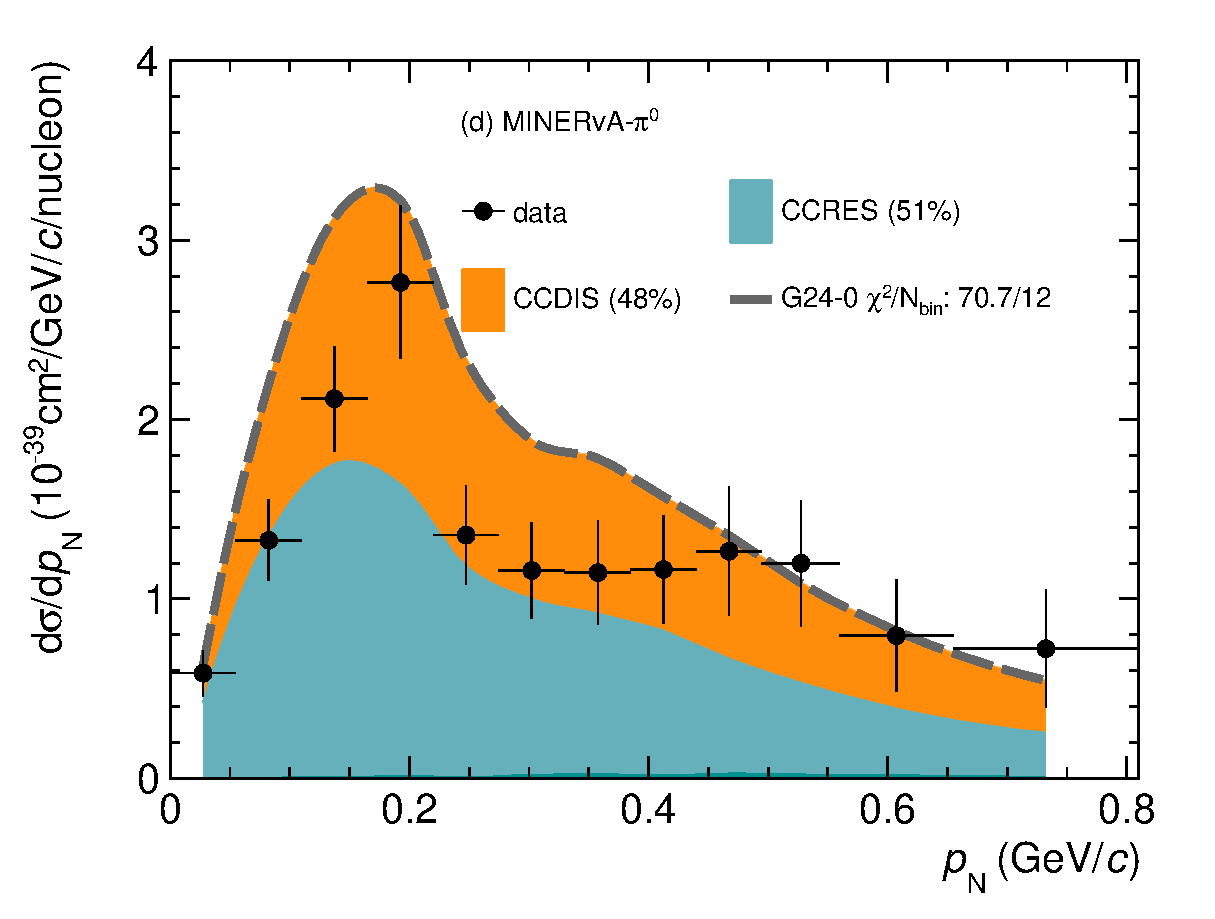
\includegraphics[width=\dbfigwid\textwidth]{figures/tuning/0000-min_pi0_pn_reac_decomp.eps}
    \caption{\label{fig:g24-0-pn-reac} Similar to Fig.~\ref{fig:g24-0-dat-reac} but for the $\pn$ (\ttkpip, \minzpi and \minpiz) and $\dpt$ (\ttkzpi) measurements.
    } 
\end{figure*}
This data-comparison shows that the model fails to describe the MINERvA $\piz$ TKI data, despite that its prediction matches other TKI data well.

As the neutrion-nucleus interacition is a complicated process, it requires multiple models to simulate the whole process, and the CMC in \genie specifies the combination of models to be used.
Tuning the entire CMC is extremely omputationally expensive, and this is the first tuning on TKI data across event topology, i.e. on both $\cczpi$ and $\cczpi$. 
Hence, before embarking on this ultimate step, it is important to first perfrom a proof-of-concept study to explore the model flexibility and to identify the most relevant model parameters.
As TKI data are sensitive to the nuclear IS and FSI, this study focuses on the tuning of these two models.
To lay the ground for better understanding of this tuning effort, I will provide a more detailed description of the inputs, i.e. the data and the models, in the following subsections. 

\subsection{The models}
\label{sec:tuning-para-choice}
    The CMCs in \genie are fomratted strings, and they are sometimes also called tunes, regardless of whether they are obtained from an actual tuning.
    The tune, \newtune, mentioned above is improved on the tune, $\geighteen$, which is obtained from the free nucleon tuning effort in Ref.~\cite{GENIE:2021zuu}, and describes bubble chamber data better.
    As \newtune\ is widely used in the paper, it will be referred to as \gZero\ for simplicity. 

    The IS in \gZero\ is modelled by the spectral-function-like Correlated Fermi Gas model (\sfcfg)~\cite{sfcfg-talk,sfcfg-GitHubCommit,GENIE:2021npt}. 
    \sfcfg\ has more adjustable parameters for tuning and improved physics compared to the local fermi gas (LFG) model used in $\geighteen$.
    The improvment arises from two aspects. 
    ``Spectral-function-like'' refers to the implementation of removal energy as a varying function rather than a fixed value, while ``Correlated'' highlights the incorporation of the high-momentum tail above the Fermi momentum due to nucleon-nucleon short-range correlations (SRC), as evidenced by electron-scattering data~\cite{CLAS:2005ola}.

    Both enhancements are incorporated into the Valencia Model (Ref.~\cite{Nieves:2004wx}).  
    Consequently, \sfcfg\ more closely reproduces the Valencia initial state than previous LFG implementations.  
    For further details on \sfcfg, see Ref.~\cite{GENIE:2021npt}.  
    Note that the original Valencia Model employs its own approach to modeling FSI. 
    However, since FSI is factorized from other processes in the \genie\ implementation, that method is not applied here.  
    Instead, GENIE has developed the INTRANUKE hA FSI model (hA for short), which is chosen as the FSI candidate for the tuning performed in this work for its simplicity and interpretability.

    Additional improvements of \gZero\ include:  
    1) adopting a $z$-expansion axial-vector form factor~\cite{Hill:2010yb} in lieu of the Valencia dipole form factor for QE processes~\cite{Nieves:2004wx}; and  
    2) substituting the Valencia model for 2p2h processes~\cite{Nieves:2011pp} with the SuSAv2 Model~\cite{Gonzalez-Jimenez:2014eqa}, which covers a broader region of the $q^0$ and $q^3$ phase space.  
    The complete list of model components is provided in Table~\ref{tab:default-gen-list}.
    \begin{table}[!htb]
        \centering
        \begin{tabular}{p{4cm}c}
        \hline
        \hline
        \textrm{Simulation component} & \textrm{Model} \\
        \hline
        \textrm{Nuclear state}              & \sfcfg~\cite{sfcfg-talk,sfcfg-GitHubCommit,GENIE:2021npt} \\ 
        \textrm{QE}               & Valencia~\cite{Nieves:2004wx} \\
        \textrm{2p2h}               & SuSAv2~\cite{Gonzalez-Jimenez:2014eqa} \\
        \textrm{QE $\Delta S=1$}           & Pais~\cite{Pais:1971er} \\
        \textrm{QE $\Delta C=1$}                  & Kovalenko~\cite{Kovalenko:1990zi} \\
        \textrm{Resonance (RES)}                        & Berger-Sehgal~\cite{Berger:2007rq}\\
        Shallow/Deep inelastic \par scattering (SIS/DIS)                    & Bodek-Yang~\cite{Bodek:2002vp}\\
        \textrm{DIS $\Delta C=1$}           & Aivazis-Tung-Olness~\cite{Aivazis:1991fy}\\
        \textrm{Coherent $\pi$ production}  & Berger-Sehgal~\cite{Berger:2008xs}\\
        \hline
        \textrm{Hadronization}              & AGKY~\cite{Yang:2009zx}\\
        \textrm{FSI}                        & INTRANUKE hA~\cite{Andreopoulos:2015wxa}\\
        \hline
        \hline
        \end{tabular}
        \caption{\label{tab:default-gen-list} Model components of \gZero\. Processes with non-trivial $\Delta S$ and $\Delta C$ are those with strangeness and charm production, respectively.}
    \end{table}
    Having selected the \gZero CMC as the tuning starting point, a closer look into the IS and FSI models, the models to be tuned, is necessary.
    The \sfcfg\ and hA model contains a total of $14$ tuneable parameters of \sfcfg\ and hA.

    The \sfcfg\ model behaviour is chiefly specified by two parameters: 
    $\srcfr$, which quantifies the fraction of the high-momentum tail from SRC above the Fermi surface, and 
    $\nurmec$, which defines the onset of the nuclear removal energy distribution for carbon.  
    A higher $\srcfr$ suggests that the initial nucleons possess greater energy, whereas a larger $\nurmec$ implies that more energy is required to liberate a nucleon, resulting in lower-energy final-state particles.  
    Due to the innovative yet loosely constrained nature of this spectral-function-like implementation, this study adopts relatively lenient priors of \(0.12\pm0.12\) for $\srcfr$ and \(0.01\pm0.005~\gev\) for $\nurmec$.

    As for the hA model~\cite{Andreopoulos:2015wxa}, its widespread use is primarily due to its straightforward reweighting capability. 
    Unlike cascade models such as the hN model~\cite{Andreopoulos:2015wxa}, the hA model assigns the FSI type for each hadron exactly once, without simulating further propagation of rescattered hadrons. 
    This single-rescattering approach is critical for interpreting tuning results. The hA model parameters are described as follows.
    \begin{enumerate}
        \item \textbf{Mean Free Path (MFP) Scaling Factors}:
        The model computes the MFP, $\lambda$, as a function of the hadron's energy, $E$, and its radial distance, $r$, from the nucleus center:
        \begin{equation}
            \lambda(E,r) = \frac{1}{\sigma_\textrm{hN,tot}(E)\rho(r)},
        \end{equation}
        where $\sigma_\textrm{hN,tot}$ is the total hadron–nucleon cross section and $\rho(r)$ is the local nucleon density. 
        Once produced within the nucleus, a hadron travels a distance $\lambda$ before a probabilistic decision on rescattering is made. 
        If no rescattering occurs, the hadron is propagated by another $\lambda$, and the process repeats until either a rescattering happens or the hadron escapes the nucleus. 
        When rescattering occurs, its type is chosen based on the relevant cross sections; the relative probabilities of these types are extracted from stored hadron scattering data~\cite{LADS:1999dyv,Navon:1983xj,Carroll:1976hj,Clough:1974qt,BAUHOFF1986429,Mashnik:2000up,Ishibashi:1997gbe}. 
        Once a specific rescattering type is determined, the resulting products are generated and considered final, with no further rescattering simulated.
        The MFPs for pions and nucleons are adjustable via scaling factors ($\cpimfp$, $\pizmfp$, and $\nmfp$) as detailed in Table~\ref{tab:hALFG-para}. 
        Due to isospin symmetry, both charged pions, $\pip$ and $\pim$, share the same scaling factor $\cpimfp$, while the $\piz$ MFP is computed from the charged pion values and adjusted separately by $\pizmfp$. 
        A scaling factor greater than unity increases $\lambda$, which in turn reduces the number of propagation steps necessary for escape and diminishes the average probability of rescattering. 
        Owing to the high precision of total hadron–nucleus cross section measurements~\cite{LADS:1999dyv,Navon:1983xj,Carroll:1976hj,Clough:1974qt,BAUHOFF1986429}, strict Gaussian priors with a standard deviation (\sigma) of 0.2 (matching the systematic uncertainties shown in Table~\ref{tab:hALFG-para}) are applied to the MFP scaling factors. 
        Notably, varying $\pizmfp$ by $\pm2.5~\sigma$ significantly affects the \minpiz\ $\textrm{d}\sigma/\textrm{d}\pn$, as illustrated in Fig.~\ref{fig:minpiz-pn-pi0mfp}. 
        In summary, a reduced MFP naturally increases rescattering, leading to fewer $\piz$s escaping the nucleus and a decreased cross section.
        \begin{figure}[!htb]
            \centering
            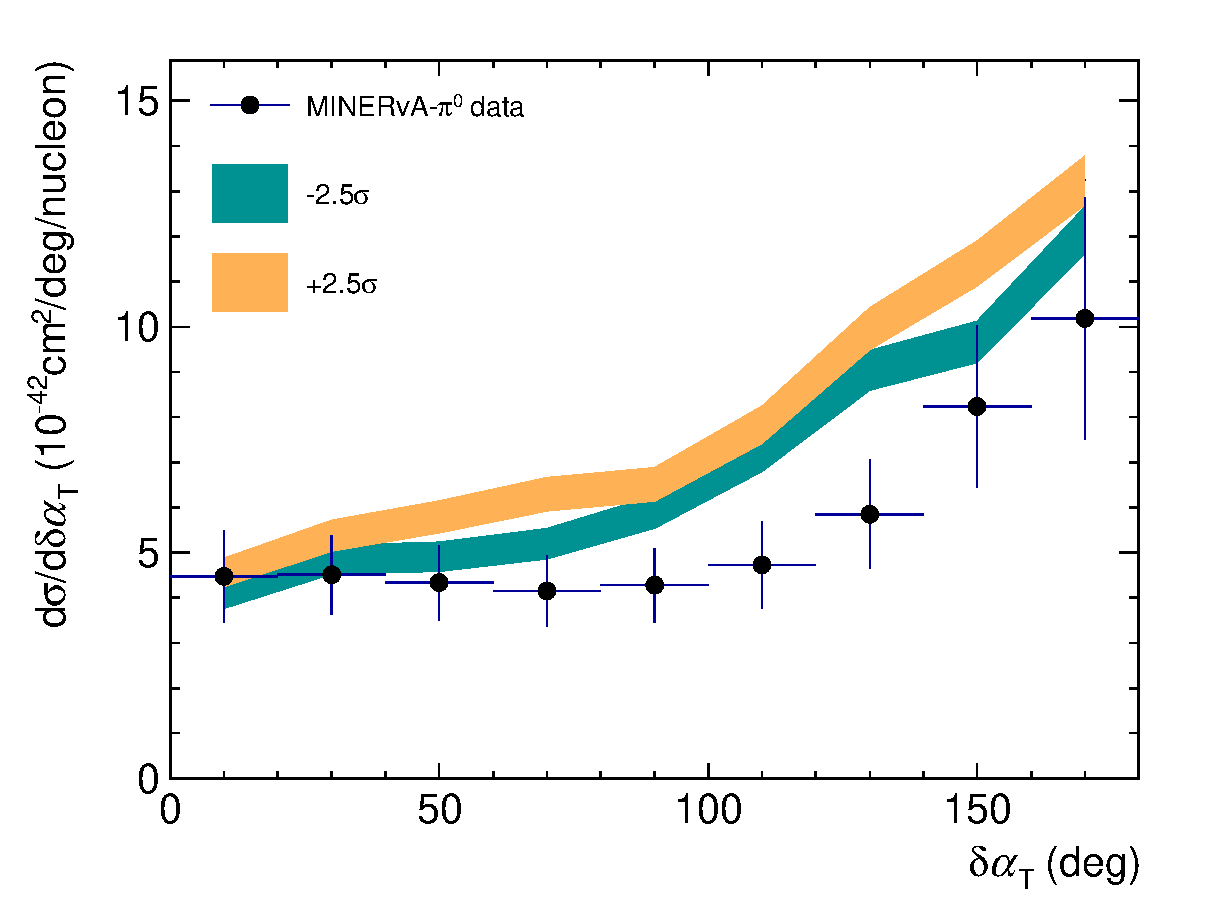
\includegraphics[width=\sgfigwid\textwidth]{figures/tuning/minerva_pi0_dalphat_FSI_pi0mfp.eps}
            \caption{Effect of varying $\pizmfp$ by $\pm2.5~\sigma$ compared to the MINERvA-$\pi^0$ measurement. Each band's width indicates the \genie prediction's statistical uncertainty from $10^5$ events.}
            \label{fig:minpiz-pn-pi0mfp}
        \end{figure}

        \item \textbf{Rescattering Type Scaling Factors}: 
        The relative probability for each rescattering type is adjusted by a scaling factor. 
        Four rescattering types are available for both nucleons and pions: charge exchange (CEX), inelastic scattering (INEL), absorption (ABS), and pion production (PIPD). 
        A detailed discussion of these tunable FSI types is provided in Sec.~\ref{sec:nuint-fsi}. 
        The default energy-dependent probability distributions, derived from hadron data tuning~\cite{LADS:1999dyv,Navon:1983xj,Carroll:1976hj,Clough:1974qt,BAUHOFF1986429}, are modified by corresponding scaling factors (e.g., $\picex$ for the CEX of all pions) as listed in Table~\ref{tab:hALFG-para}. 
        After scaling, the probabilities are renormalized so that they sum to one. 
        For instance, if the initial absorption fraction, $f_\textrm{ABS}$, is 0.5 (with the remaining fraction, $f_\textrm{other}=f_\textrm{INEL}+f_\textrm{CEX}+f_\textrm{PIPD}$, also 0.5), scaling $f_\textrm{ABS}$ by $S_\textrm{ABS}=2$ yields
        \begin{equation}
            f^\prime_\textrm{ABS} = \frac{f_\textrm{ABS} \cdot S_\textrm{ABS}}{f_\textrm{ABS} \cdot S_\textrm{ABS}+f_\textrm{other}} = \frac{2}{3},
        \end{equation}
        illustrating that the effective increase in $f_\textrm{ABS}$ is less than the scaling factor alone due to normalization with the other FSI types.
        Here, $f_\textrm{ABS}$ is effectively scaled by a factor of 1.3 rather than 2. 
        Therefore, a relatively relaxed Gaussian prior with a $\sigma$ of 0.5 is imposed on the FSI fate scales, slightly exceeding the systematic uncertainties in Table~\ref{tab:hALFG-para}.
        A side-effect due to this normalization is that changing one scaling factor inherently affects the others.
        In practice, plotting the cross section by rescattering type clarifies the net changes.
    \end{enumerate}
    
    Table~\ref{tab:hALFG-para} summarizes the tuneable parameters and their ranges imposed in tuning.
    Nominal values and associated uncertainties for the hA model are taken from Table 17.3 in Ref.~\cite{Andreopoulos:2015wxa}. 
    \begin{table}[!htb]
        \centering
        \begin{tabular}{ccccc}
        \hline
        \hline
        \textrm{Parameter} & \textrm{Nominal} (\gZero)     & \textrm{Range In} \textrm{Tuning} & \allpar (\gT)  & \redpar (\gC) \\ 
        \hline
        \multicolumn{5}{c}{\sfcfg} \\
        \hline
        \textrm{$\srcfr$} & 0.12 & (0.0, 0.5)  & \tick & \tick\\
        \textrm{$\nurmec$} & 0.01 & (0.0, 0.2) & \tick & \\
        \hline
        \multicolumn{5}{c}{hA} \\
        \hline
        \textrm{$\cpimfp$} & $1.0\pm0.2$ & (0.0, 3.0) & \tick & \\
        \textrm{$\pizmfp$} & $1.0\pm0.2$ & (0.0, 3.0) & \tick & \tick\\
        \textrm{$\nmfp$} & $1.0\pm0.2$ & (0.0, 3.0) & \tick &\\
        \hline
        \textrm{$\picex$} &  $1.0\pm0.5$ & (0.0, 3.0) & \tick & \tick \\
        \textrm{$\ncex$} & $1.0\pm0.5$ & (0.0, 3.0)  & \tick & \tick\\
        \hline
        \textrm{$\piinel$} & $1.0\pm0.4$ & (0.0, 3.0) & \tick & \\
        \textrm{$\ninel$} & $1.0\pm0.4$ & (0.0, 3.0)  & \tick &\\
        \hline
        \textrm{$\cpiabs$} & $1.0\pm0.2$ & (0.0, 3.0) & \tick &\\
        \textrm{$\pizabs$} & $1.0\pm0.2$ & (0.0, 3.0) & \tick &\\
        \textrm{$\nabs$} & $1.0\pm0.2$ & (0.0, 3.0)  & \tick & \tick\\
        \hline
        \textrm{$\pipiprod$} & $1.0\pm0.2$ & (0.0, 3.0) & \tick &\\
        \textrm{$\npiprod$} & $1.0\pm0.2$ & (0.0, 3.0)  & \tick & \tick\\
        \hline
        \hline
        \end{tabular}
        \caption{\label{tab:hALFG-para}
        Tuneable parameters and their ranges in the  \sfcfg\ (\textit{uppermost} group) and hA (\textit{lower} groups, uncertainties from Ref.~\cite{Andreopoulos:2015wxa}) models. Parameters to be tuned in the two sets are marked with ``\tick'''s. See later text for definitions of \gT and \gC.
        }
    \end{table}

    \subsection{The data}
    Not only the \minpiz data set, where the discrepancy lies, is used for tuning, but the other three data sets are also included, as it is important to maintain the good data-MC agreement for the existing data sets, while improving the agreement for the \minpiz data set.

    The common requirement of the four measurements is the presence of one CC muon and at least one proton in the final state. 
    The $0\pi$ data sets, i.e. \ttkzpi and \minzpi, require the absence of any pions, while \ttkpip\ requires exactly one $\pi^+$, and \minpiz\ requires at least one $\pi^0$.
    The four data sets further differ slightly in the kinematic cuts, as summarized in Table~\ref{tab:data-sets-phase-space-cut}, and they also contain slightly different combinations of the TKI variables, as detailed in Table~\ref{tab:data-sets}.
    \begin{table}[!htb]
        \centering
        \begin{tabular}{cc}
        \hline
        \hline
        Variables & Cuts ($p$ in $\gevc$) \\
        \hline
        \multicolumn{2}{c}{\ttkzpi~\cite{T2K:2018rnz}} \\
        \hline
        $\vecpmu$    &  $0.25 < p_\mu $, $\cos\theta_\mu>-0.6$   \\
        $\vecpp$     & $0.45< p_\text{p} <1.0$ , $\cos\theta_\text{p}>0.4$     \\
        \hline
        \multicolumn{2}{c}{\ttkpip~\cite{T2K:2021naz}} \\
        \hline
        $\vecpmu$    & $0.25 < p_\mu < 7$ , $\theta_\mu < 70^\degree$  \\
        $\vecpp$     & $0.45 < p_\text{p} <1.2$  ,  $\theta_\text{p} < 70^\degree$   \\
        $\vecppi$    & $0.15 < p_\pi <  1.2$, $\theta_\pi < 70^\degree$ \\
        \hline
        \multicolumn{2}{c}{\minzpi~\cite{MINERvA:2018hba, MINERvA:2019ope}} \\
        \hline
        $\vecpmu$     & $1.5< p_\mu < 10$ , $\theta_\mu < 20^\degree $  \\
        $\vecpp$      & $0.45< p_\text{p} <1.2$  , $\theta_\text{p} < 70^\degree$    \\
        \hline
        \multicolumn{2}{c}{\minpiz~\cite{MINERvA:2020anu}} \\
        \hline
        $\vecpmu$   & $1.5< p_\mu < 20$ , $\theta_\mu < 25^\degree$  \\
        $\vecpp$    & $0.45< p_\text{p} $                      \\
        \hline
        \hline
        \end{tabular}
        % \end{ruledtabular}
        \caption{\label{tab:data-sets-phase-space-cut}
        Kinematic cuts for the samples of the TKI measurements.
        }
    \end{table}

    As not all TKI observables are linearly indepedent, such as $\dpt$ and $\pn$, and some might have strong dependence outside IS and FSI, such as $\dphit$ displaying a strong dependence on neutrino beam energy~\cite{Lu:2015tcr}, it might be redundant and ineffective to include all of them in the tuning.
    In order to discern the most sensitive observables, a systematic evaluation of various combinations of observables was undertaken for the tuning process. 
    A total of 26 combinations, as shown in Table~\ref{tab:fit-var-combo}, are examined. 
    These combinations are formed according to the following patterns:
    \begin{itemize}
        \item \textbf{\texttt{Combi-}1 through 5} are cross-experiment selections of a single observable. 
        For example, \texttt{Combi-}$3$ uses only $\dat$ from all four data sets. 
        If a chosen observable is absent from a dataset, that dataset is excluded from the specific combination. 
        For example, \ttkzpi is not used in \texttt{Combi-}1 due to the absence of $\pn$.
        \item \textbf{\texttt{Combi-}6 through 9} incorporate all variables from a single measurement. For example, \texttt{Combi-}$9$ uses \minpiz only.
        \item \textbf{\texttt{Combi-}10 to 13} uses two out of four measurements according to the experiment or topology. For example, \texttt{Combi-}$10$ uses only the two data sets from T2K, and \texttt{Combi-}$13$  only with pion production. 
        \item \textbf{\texttt{Combi-}14 to 17} are cross-experiment selections of two observables. 
        For example, \texttt{Combi-14} uses all $\dat$ and $\dptt$ measurements across all data sets, while \texttt{Combi-17} uses $\dat$ and $\dpt$.
        \item \textbf{\texttt{Combi-}18 through 22} are cross-experiment selections of three observables. 
        For example, \texttt{Combi-18} uses all available $\dat$, $\dptt$, and $\pn$, while \texttt{Combi-22} uses $\dpt$, $\dphit$, and $\pn$.
        \item \textbf{\texttt{Combi-}23} uses all observables except $\dphit$ from all data sets.
        \item \textbf{\texttt{Combi-}24} encompasses all variables, acting as the superset.
        \item \textbf{\texttt{Combi-}25 and 26} are the same as \texttt{Combi-}$21$ and $23$, respectively, except that $\dpt$ in \minzpi is removed to avoid correlation with $\pn$ in the same data set.
    \end{itemize}

    \begin{table}[h]
    \begin{tabular}{l|lllll|llll|llll|lp{1cm}ll|lllll|l|p{1cm}|lp{1cm}}
    \hline
    \hline
    \texttt{Combi-}        & 1 & 2 & 3 & 4 & 5 & 6 & 7 & 8 & 9 & 10 & 11 & 12 & 13 & 14 & 15 \par (\texttt{Best-}\par\allpar) & 16 & 17 & 18 & 19 & 20 & 21 & 22 & 23 & 24 \par (\texttt{Super-}\par\texttt{set}) & 25 & 26 \par (\texttt{Best-}\par\redpar)\\
            \hline
    \multicolumn{27}{c}{\ttkzpi} \\
    \hline
    $\dat$      &   &   & $\tick$ &   &   & $\tick$ &   &   &   & $\tick$  &    & $\tick$  &    & $\tick$  &    & $\tick$  & $\tick$  & $\tick$  & $\tick$  & $\tick$  & $\tick$  &    & $\tick$  & $\tick$  & $\tick$  & $\tick$  \\
    $\dpt$   &   & $\tick$ &   &   &   & $\tick$ &   &   &   & $\tick$  &    & $\tick$  &    &    & $\tick$  &    & $\tick$  &    & $\tick$  &    & $\tick$  & $\tick$  & $\tick$  & $\tick$  & $\tick$  & $\tick$  \\
    $\dphit$ &   &   &   & $\tick$ &   & $\tick$ &   &   &   & $\tick$  &    & $\tick$  &    &    &    &    &    &    &    & $\tick$  &    & $\tick$  &    & $\tick$  &    &    \\
    \hline
    \multicolumn{27}{c}{\ttkpip} \\
    \hline
    $\dat$      &   &   & $\tick$ &   &   &   & $\tick$ &   &   & $\tick$  &    &    & $\tick$  & $\tick$  &    & $\tick$  & $\tick$  & $\tick$  & $\tick$  & $\tick$  & $\tick$  &    & $\tick$  & $\tick$  & $\tick$  & $\tick$  \\
    $\pn$       & $\tick$ &   &   &   &   &   & $\tick$ &   &   & $\tick$  &    &    & $\tick$  &    & $\tick$  & $\tick$  &    & $\tick$  &    &    & $\tick$  & $\tick$  & $\tick$  & $\tick$  & $\tick$  & $\tick$  \\
    $\dptt$     &   &   &   &   & $\tick$ &   & $\tick$ &   &   & $\tick$  &    &    & $\tick$  & $\tick$  &    &    &    & $\tick$  & $\tick$  & $\tick$  &    &    & $\tick$  & $\tick$  &    & $\tick$  \\
    \hline
    \multicolumn{27}{c}{\minzpi} \\
    \hline
    $\dat$      &   &   & $\tick$ &   &   &   &   & $\tick$ &   &    & $\tick$  & $\tick$  &    & $\tick$  &    & $\tick$  & $\tick$  & $\tick$  & $\tick$  & $\tick$  & $\tick$  &    & $\tick$  & $\tick$  & $\tick$  & $\tick$  \\
    $\pn$       & $\tick$ &   &   &   &   &   &   & $\tick$ &   &    & $\tick$  & $\tick$  &    &    & $\tick$  & $\tick$  &    & $\tick$  &    &    & $\tick$  & $\tick$  & $\tick$  & $\tick$  & $\tick$  & $\tick$  \\
    $\dpt$      &   & $\tick$ &   &   &   &   &   & $\tick$ &   &    & $\tick$  & $\tick$  &    &    & $\tick$  &    & $\tick$  &    & $\tick$  &    & $\tick$  & $\tick$  & $\tick$  & $\tick$  &    &    \\
    $\dphit$    &   &   &   & $\tick$ &   &   &   & $\tick$ &   &    & $\tick$  & $\tick$  &    &    &    &    &    &    &    & $\tick$  &    & $\tick$  &    & $\tick$  &    &    \\
    \hline
    \multicolumn{27}{c}{\minpiz} \\
    \hline
    $\dat$      &   &   & $\tick$ &   &   &   &   &   & $\tick$ &    & $\tick$  &    & $\tick$  & $\tick$  &    & $\tick$  & $\tick$  & $\tick$  & $\tick$  & $\tick$  & $\tick$  &    & $\tick$  & $\tick$  & $\tick$  & $\tick$  \\
    $\pn$       & $\tick$ &   &   &   &   &   &   &   & $\tick$ &    & $\tick$  &    & $\tick$  &    & $\tick$  & $\tick$  &    & $\tick$  &    &    & $\tick$  & $\tick$  & $\tick$  & $\tick$  & $\tick$  & $\tick$  \\
    $\dptt$     &   &   &   &   & $\tick$ &   &   &   & $\tick$ &    & $\tick$  &    & $\tick$  & $\tick$  &    &    &    & $\tick$  & $\tick$  & $\tick$  &    &    & $\tick$  & $\tick$  &    & $\tick$ \\
    \hline
    \hline    
    \end{tabular}
    \caption{\label{tab:fit-var-combo}
    Specifications of observable combinations within the tuning superset in Table~\ref{tab:data-sets}. \texttt{Combi-15} is \texttt{Best-}\allpar, \texttt{Combi-24} is \texttt{Superset}, and \texttt{Combi-26} is \texttt{Best-}\redpar. 
    }
    \end{table}

    For each combination, variables omitted from tuning—including proton momentum and angle ($p_\text{p}$ and $\theta_\text{p}$)~\cite{MINERvA:2018hba}, as well as $\dptx$ and $\dpty$~\cite{MINERvA:2019ope} in \minzpi—were reserved solely for validation; the expectation is that the model will accurately reproduce these observables following tuning. 
    To identify the optimal combination, this study employs a criterion based on the $\chi^2$ calculated over the complete (tuned plus validation) observable set.
    Figure~\ref{fig:allchi} shows the change in $\chi^2$ for the complete observable set as for each tuning combination, where the two sets of model parameters, \allpar and \redpar, are compared. 
    The respective minima happen at \texttt{Combi-15} and 26. 


\begin{table}[!htb]
    \centering
    \begin{tabular}{ccccc}
    \hline
    \hline
    Observables & No. of bins & \texttt{Combi-} \texttt{Superset}  & \texttt{Combi-} \texttt{Best-} \allpar& \texttt{Combi-} \texttt{Best-} \redpar\\
    \hline
    \multicolumn{5}{c}{\ttkzpi} \\
    \hline
       $\dat$            & $8$                & $\tick$     &          & $\tick$  \\ 
       $\dpt$            & $8$                & $\tick$     &          & $\tick$ \\ 
       $\dphit$          & $8$                & $\tick$     &          &  \\      
    \hline
    \multicolumn{5}{c}{\ttkpip} \\
    \hline
      $\dat$            & $3$                & $\tick$      & $\tick$  & $\tick$  \\
      $\pn$             & $4$                & $\tick$      & $\tick$  & $\tick$ \\ 
      $\dptt$           & $5$                & $\tick$      & $\tick$  & $\tick$  \\ 
    \hline
    \multicolumn{5}{c}{\minzpi} \\
    \hline  
      $\dat$            & $12$               & $\tick$      &          & $\tick$  \\ 
      $\pn$             & $24$               & $\tick$      &          & $\tick$ \\
      $\dpt$            & $24$               & $\tick$      &          &  \\     
      $\dphit$          & $23$               & $\tick$      &  &  \\     
      $\pp$             & $25$               &      &  &  \\     
      $\thetap$         & $26$               &      &  &  \\     
      $\dptx$           & $32$               &      &  &  \\  
      $\dpty$           & $33$               &      &  & \\     
    \hline
    \multicolumn{5}{c}{\minpiz} \\
    \hline
      $\dat$            & $9$               & $\tick$      & $\tick$   & $\tick$      \\  
      $\pn$             & $12$               & $\tick$     & $\tick$  & $\tick$ \\ 
      $\dptt$           & $13$               & $\tick$     & $\tick$  & $\tick$  \\   \hline
    \hline
    \end{tabular}
    \caption{\label{tab:data-sets}
	(NEW) Observables of the TKI measurements and their binning. Those with ``$\tick$'''s are used for tuning, while those without  are for the respective validation. See Table~\ref{tab:hALFG-para} for definitions of \cbRedPar and \cbAllPar.
    }
\end{table}



\begin{figure}[!htb] 
    \centering 		
    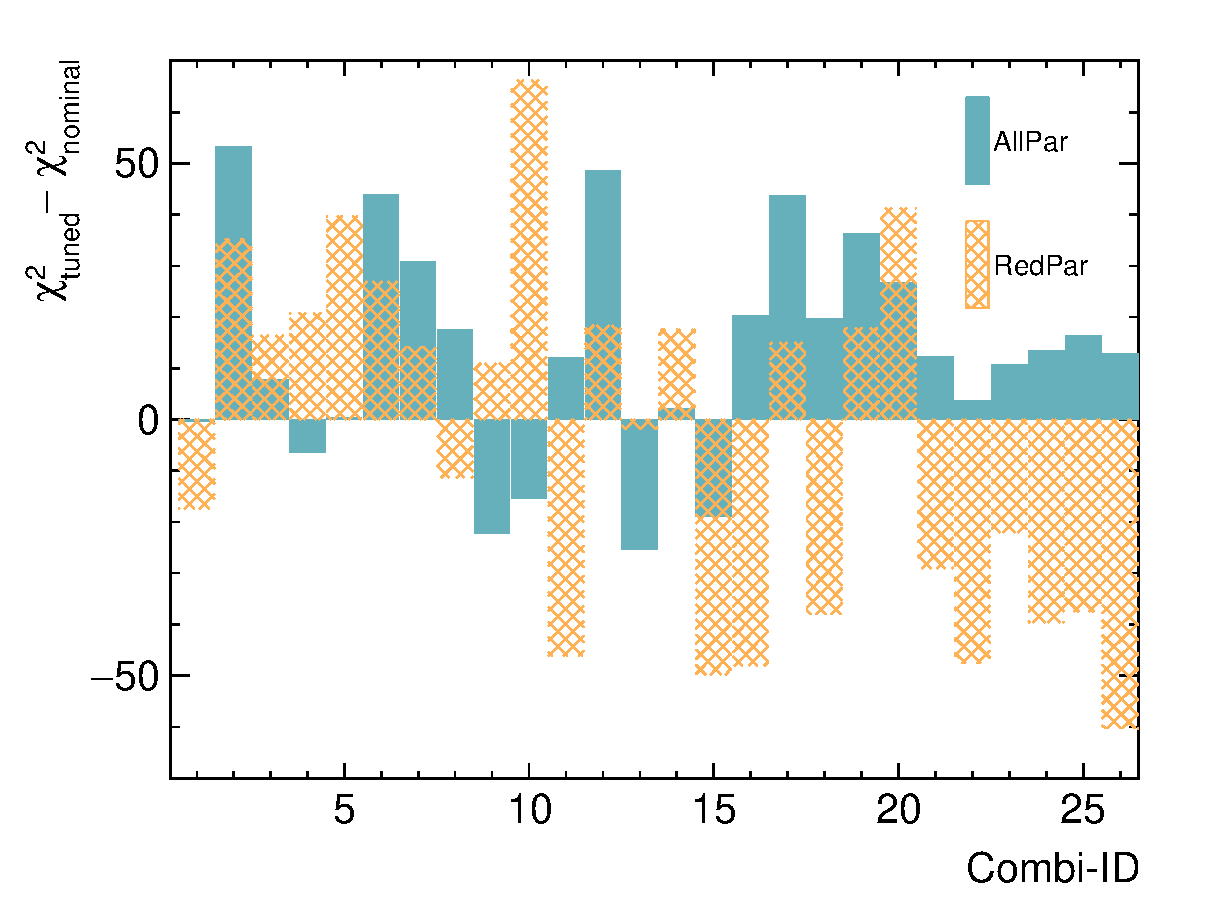
\includegraphics[width=\sgfigwid\textwidth]{figures/tuning/chi2_hist_covfix.eps} 
    \caption{\label{fig:allchi} Change of $\chi^2$ calculated for the full (i.e., tuned plus validation) observable set as a function of the tuned combination (cf. Table~\ref{tab:fit-var-combo} in Appendix~\ref{sec:appcombi}). The two model parameter sets (\allpar and \redpar, see Table~\ref{tab:hALFG-para} for definitions) are compared and it can be seen that the respective minima happen at \texttt{Combi-13} and 26. }   
\end{figure}

%========= old ===================
The GENIE collaboration has demonstrated successful tuning of the various components of the neutrino-nucleus interaction model. 
For instance, 

The large data samples and superb imaging capabilities of modern neutrino experiments offer us a detailed new look at neutrino interaction physics. 
Recently, the GENIE~\cite{Andreopoulos:2009rq, GENIE:2021npt} Collaboration has made substantial progress towards a global tuning using neutrino, charged lepton, and hadron scattering data, in an attempt to integrate new experimental constraints with state-of-the-art theories and construct robust and comprehensive simulations of neutrino interactions with matter. 
Cross-experiment and cross-topology analyses are challenging tasks as each measurement features its unique selection criteria and various other aspects, such as the neutrino flux. 
\genie has built an advanced tuning framework that enables the validation and tuning of comprehensive interaction models using an extensive curated database of measurements of neutrino, charged lepton, and hadron scattering off nucleus and nuclei. 
So far, the non-resonant backgrounds~\cite{GENIE:2021zuu}, hadronization~\cite{GENIE:2021wox}, and the quasielastic (QE) and 2-particle-2-hole (2p2h) components~\cite{GENIE:2022qrc} of the neutrino-nucleus interaction have been tuned with $\nu_\mu$ and $\bar{\nu}_\mu$ charged-current (CC) pionless (0$\pi$) data from MiniBooNE, T2K, and MINERvA. 
A partial tune was performed for each experiment, highlighting the neutrino energy dependence on the QE and 2p2h tuned cross sections. 
Even though post-tune predictions enhanced the data description for each experiment, the added degrees of freedom were not sufficient to fully describe all CC0$\pi$ data and exhibited tensions with some proton observables~\cite{GENIE:2022qrc}. 
More exclusive measurements result in additional model constraints. 
In addition, observables that are sensitive to targeted aspects of the complex dynamics of neutrino interactions are invaluable for model tuning. 
The transverse kinematic imbalance (TKI)~\cite{Lu:2015hea, Lu:2015tcr}, a final-state correlation between the CC lepton and the hadronic system, is a good example since it is sensitive to the initial-state nuclear environment and hadronic FSI. 
Our next step is to incorporate TKI data from experiments where various exclusive topologies at different energies are considered. 
This marks the first combined tuning on TKI data with and without pions in the final states and serves as the starting point of a more comprehensive tuning effort in the energy region most relevant for future accelerator-based neutrino experiments.  

This chapter is structured as follows: 
Sec.~\ref{sec:genie} reviews the \genie models, and Sec.~\ref{sec:Tuning} details the tuning considerations and procedures. 
Results are summarized in Sec.~\ref{sec:results}, highlighting how the data-MC discrepancy in the \minpiz\ TKI measurement~\cite{MINERvA:2020anu} is resolved while maintaining good data-MC agreement elsewhere. 
The last section summarises the chapter and outlines future work.

The definitions of the kinematic cuts for these samples are summarized in Table~\ref{tab:data-sets-phase-space-cut}. 



\section{\genie Model Selection and Configuration}\label{sec:genie}
% \genie uses formatted strings to uniquely define configurations, which are usually called tunes. 
% Regardless of the name, they can refer to configurations either before or after an actual tuning procedure. 

% Free nucleon tuning effort in Ref.~\cite{GENIE:2021zuu} has produced a tune, $\geighteen$, with better description of bubble chamber data. 
% This is the starting point of the model we want to tune. 
% The first effect to apply to this model is adding the proper initial state. 
% Among the available \genie initial state models, the best choice is the spectral-function-like Correlated Fermi Gas model (\sfcfg)~\cite{sfcfg-talk,sfcfg-GitHubCommit,GENIE:2021npt}. 
% \sfcfg\ is essentially based on the previously implemented Local Fermi Gas (LFG) model in \genie with a larger number of adjustable degrees of freedom for tuning and improved physics. 
% It differs from the previous implementation of LFG in two aspects. 
% ``Spectral-function-like'' refers to the implementation of removal energy as a varying function rather than a fixed value, while ``Correlated'' highlights the incorporation of the high-momentum tail above the Fermi momentum due to nucleon-nucleon short-range correlations (SRC), as evidenced by electron-scattering data~\cite{CLAS:2005ola}.
% These two improvements are considered and modeled in the Valencia Model in Ref.~\cite{Nieves:2004wx}.
% Hence, \sfcfg\ resembles closer the initial state of the Valencia model than previous LFG implementations.
% More details on the \sfcfg\ can be found in Ref.~\cite{GENIE:2021npt}. 
% Note that the original Valencia Model in Ref.~\cite{Nieves:2004wx} has its own method of modeling FSI. 
% However, since FSI is factorized from other models in implementation in \genie, this method is not used.
% Instead, GENIE develops the INTRANUKE hA FSI model (hA for short) for its simplicity and interpretability, which is the FSI candidate for the model to be tuned in this work.

% Further improvements to the configuration to be tuned include: 1) using $z$-expansion axial-vector form factor~\cite{Hill:2010yb} rather than the dipole form factor of the Valencia model in QE processes~\cite{Nieves:2004wx}; and 2) replacing the Valencia model~\cite{Nieves:2011pp} in 2p2h processes with the SuSAv2 Model~\cite{Gonzalez-Jimenez:2014eqa} since it covers larger region of the $q^0$, $q^3$ phase space.

%\sout{Given its simplicity and interpretability, the INTRANUKE hA FSI model (hA for short) emerges as the FSI candidate for the model to be tuned.}
% The complete list of the model components are given in Table ~\ref{tab:default-gen-list}. 
% In the \genie code, this configuration is identified as \newtune\ and it is currently the default \genie configuration for a number of LAr based experiments. 
% As \newtune\ is widely used in the paper, we will call it \gZero\ for simplicity. 

% Comparing the \genie predictions for \gZero\ against TKI datasets, Figs.~\ref{fig:g24-0-dat-reac} and~\ref{fig:g24-0-pn-reac},  shows that the model fails to accurately describe the MINERvA $\pi^0$ TKI measurement~\cite{MINERvA:2020anu}. 

% \begin{table}[!htb]
%     \centering
%     \begin{tabular}{p{4cm}c}
%     \hline
%     \hline
%     \textrm{Simulation component} & \textrm{Model} \\
%     \hline
%     \textrm{Nuclear state}              & \sfcfg~\cite{sfcfg-talk,sfcfg-GitHubCommit,GENIE:2021npt} \\ 
%     \textrm{QE}               & Valencia~\cite{Nieves:2004wx} \\
%     \textrm{2p2h}               & SuSAv2~\cite{Gonzalez-Jimenez:2014eqa} \\
%     \textrm{QE $\Delta S=1$}           & Pais~\cite{Pais:1971er} \\
%     \textrm{QE $\Delta C=1$}                  & Kovalenko~\cite{Kovalenko:1990zi} \\
%     \textrm{Resonance (RES)}                        & Berger-Sehgal~\cite{Berger:2007rq}\\
%     Shallow/Deep inelastic \par scattering (SIS/DIS)                    & Bodek-Yang~\cite{Bodek:2002vp}\\
%     \textrm{DIS $\Delta C=1$}           & Aivazis-Tung-Olness~\cite{Aivazis:1991fy}\\
%     \textrm{Coherent $\pi$ production}  & Berger-Sehgal~\cite{Berger:2008xs}\\
%     \hline
%     \textrm{Hadronization}              & AGKY~\cite{Yang:2009zx}\\
%     \textrm{FSI}                        & INTRANUKE hA~\cite{Andreopoulos:2015wxa}\\
%     \hline
%     \hline
%     \end{tabular}
%     \caption{\label{tab:default-gen-list} Model components of \gZero\. Processes with non-trivial $\Delta S$ and $\Delta C$ are those with strangeness and charm production, respectively.}
% \end{table}




\subsection{\label{sec:tuning-obs-choice} Data points}
% The observables for the reported differential cross sections across the four TKI measurements---\ttkzpi, \ttkpip, \minzpi, and \minpiz---are detailed in Table~\ref{tab:data-sets}. 
% To identify the most sensitive variables, various combinations were evaluated for tuning purposes. 
% A total of 26 combinations were assessed,  with the superset comprising $\dat$, $\dpt$, $\dphit$, $\pn$, and $\dptt$ (see Table~\ref{tab:fit-var-combo} in Appendix~\ref{sec:appcombi} for all combinations). 
% Each combination was evaluated such that non-selected variables---including proton momentum and angle ($p_\text{p}$ and $\theta_\text{p}$)~\cite{MINERvA:2018hba}, as well as $\dptx$ and $\dpty$~\cite{MINERvA:2019ope} in \minzpi---were used solely for validation; the model is expected to accurately predict these variables post-tuning. 
% When constructing the combinations, it was observed that $\dphit$ is strongly dependent  on neutrino beam energy~\cite{Lu:2015tcr}, which suppresses its sensitivity to nuclear effects. 
% Additionally, correlations exist between various observables, notably between $\dpt$ and $\pn$. 
% Therefore, determining the optimal combination is not straightforward; this study employs a criterion based on  the $\chi^2$ with the complete (tuned plus validation) observable set (Fig.~\ref{fig:allchi}).




\section{\label{sec:results}The first TKI-driven \genie tunes}

% \begin{figure}[!htb] 	
%     \centering 		
%     \begin{subfigure}{width=\dbfigwid\textwidth}
%     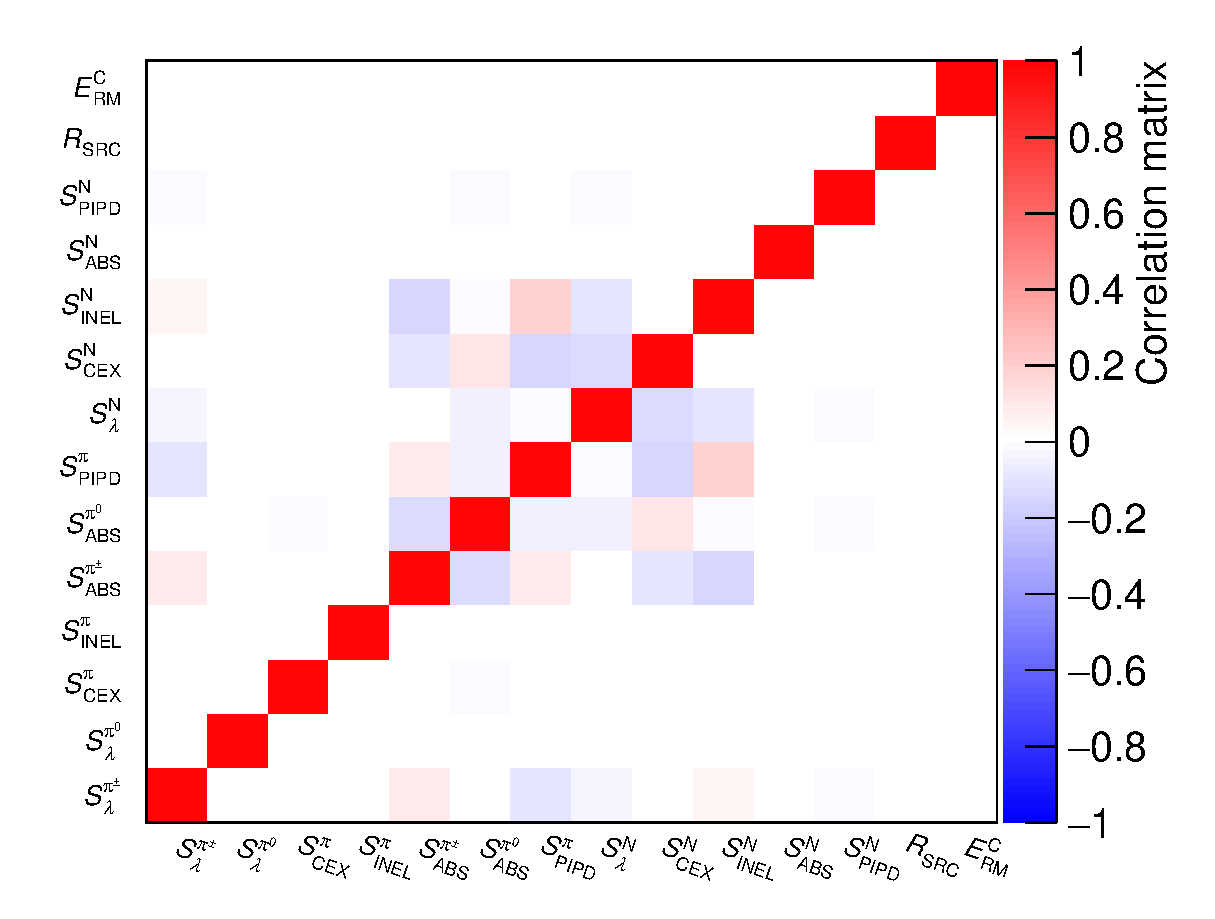
\includegraphics{figures/tuning/result_test_comb_26_cor_allpar_covfix.eps}
%     \subcaption{\label{fig:comb_26_cor_allpar}\allpar}
%     \end{subfigure}
%     \begin{subfigure}{width=\dbfigwid\textwidth}
%     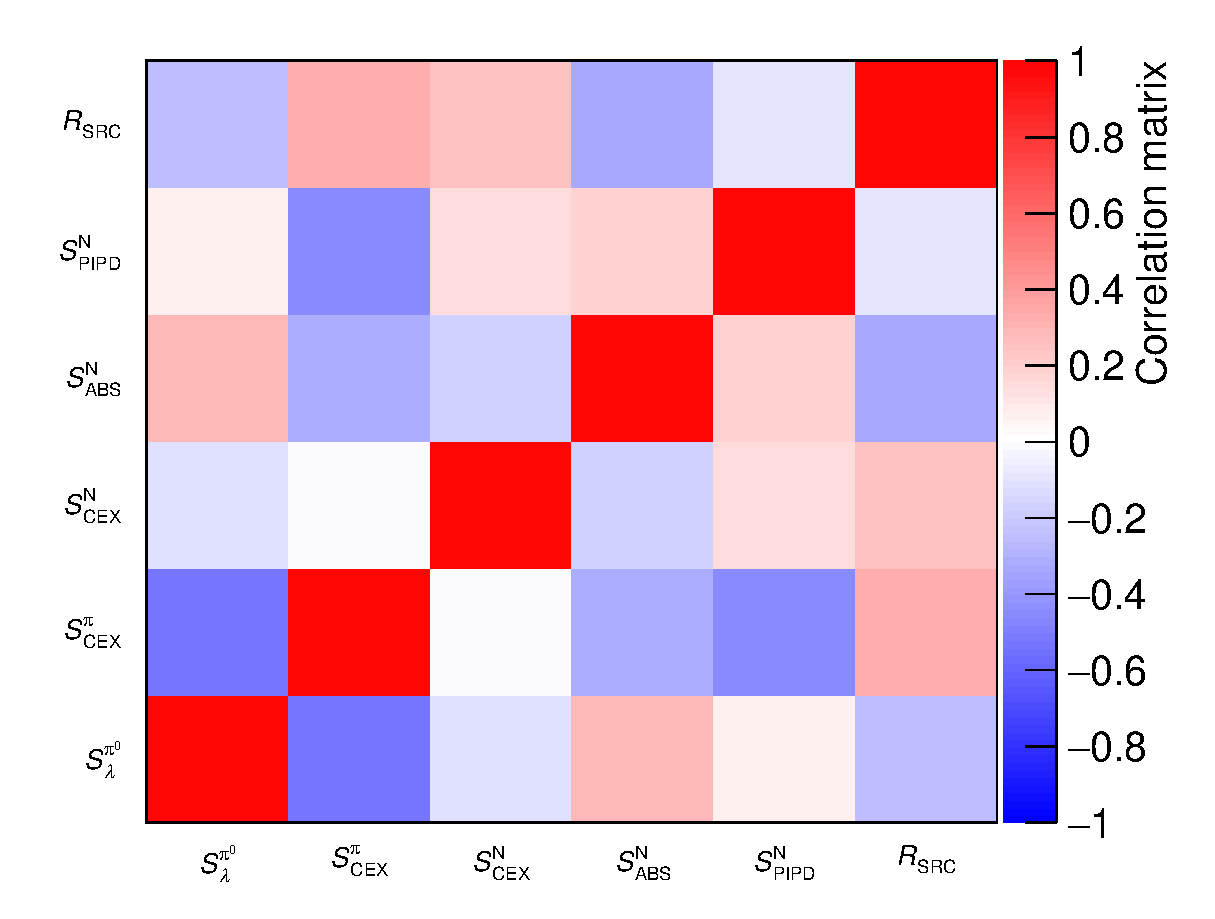
\includegraphics{figures/tuning/result_test_comb_26_cor_redpar_covfix.eps}
%     \subcaption{\label{fig:comb_26_cor_redpar}\redpar}
%     \end{subfigure}
%     \caption{ Post-fit Correlation coefficient on \texttt{Combi-26}. } 
% \end{figure}

\begin{figure}[!htb] 	
    \centering 		
    \begin{subfigure}{\dbfigwid\textwidth}
        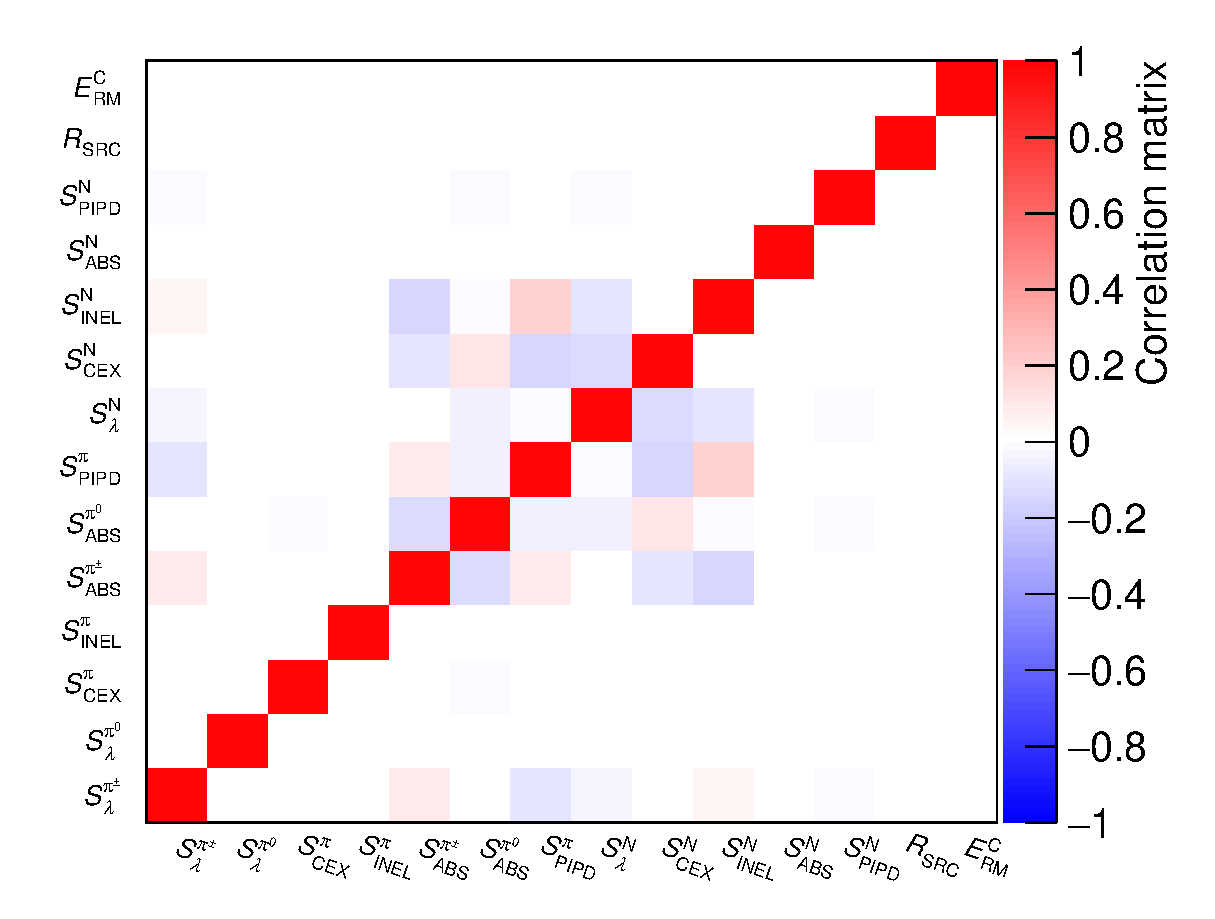
\includegraphics[width=\textwidth]{figures/tuning/result_test_comb_26_cor_allpar_covfix.eps}
        \caption{\allpar}
        \label{fig:comb_26_cor_allpar}
    \end{subfigure}
    \begin{subfigure}{\dbfigwid\textwidth}
        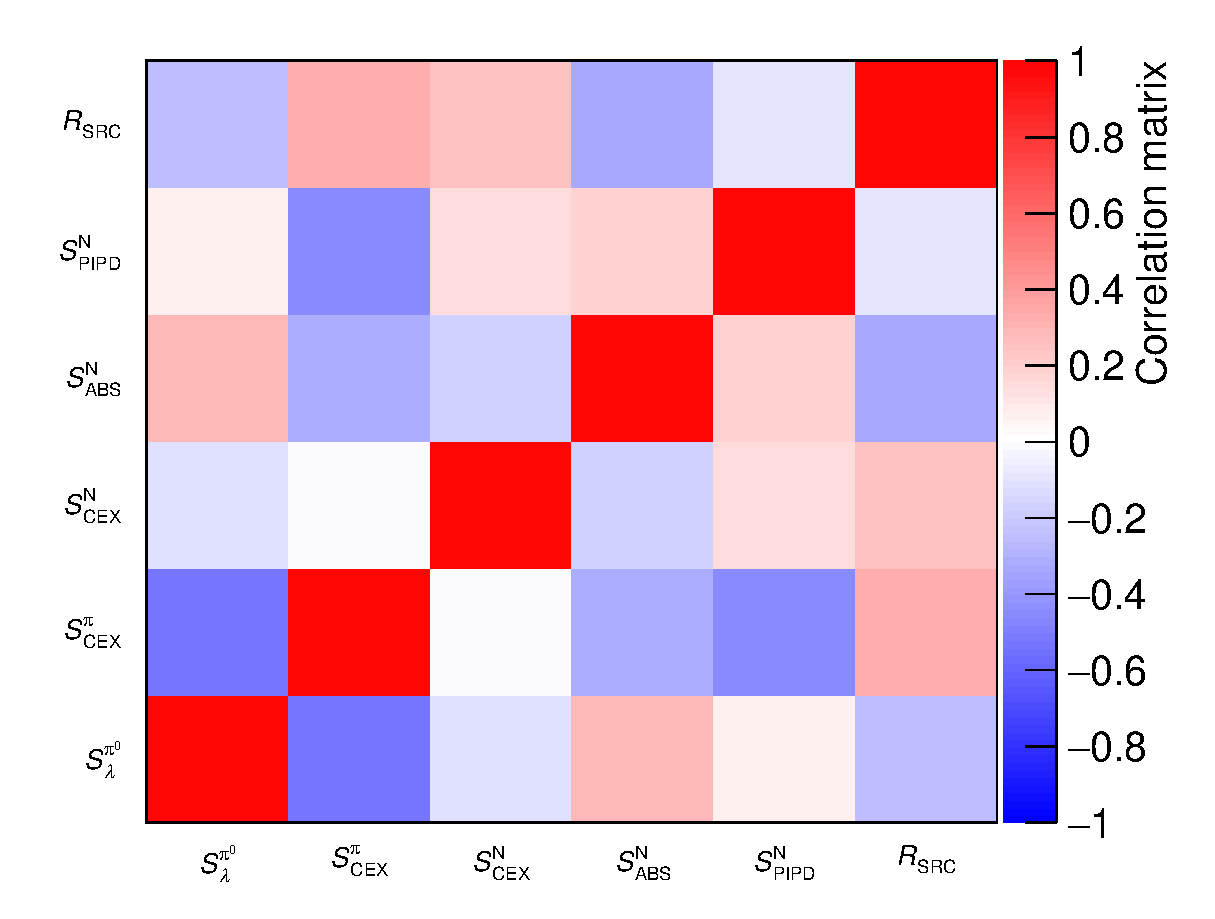
\includegraphics[width=\textwidth]{figures/tuning/result_test_comb_26_cor_redpar_covfix.eps}
        \caption{\redpar}
        \label{fig:comb_26_cor_redpar}
    \end{subfigure}
    \caption{ Post-fit Correlation coefficient on \texttt{Combi-26}. } 
\end{figure}

\begin{figure*} 
    \centering 		
    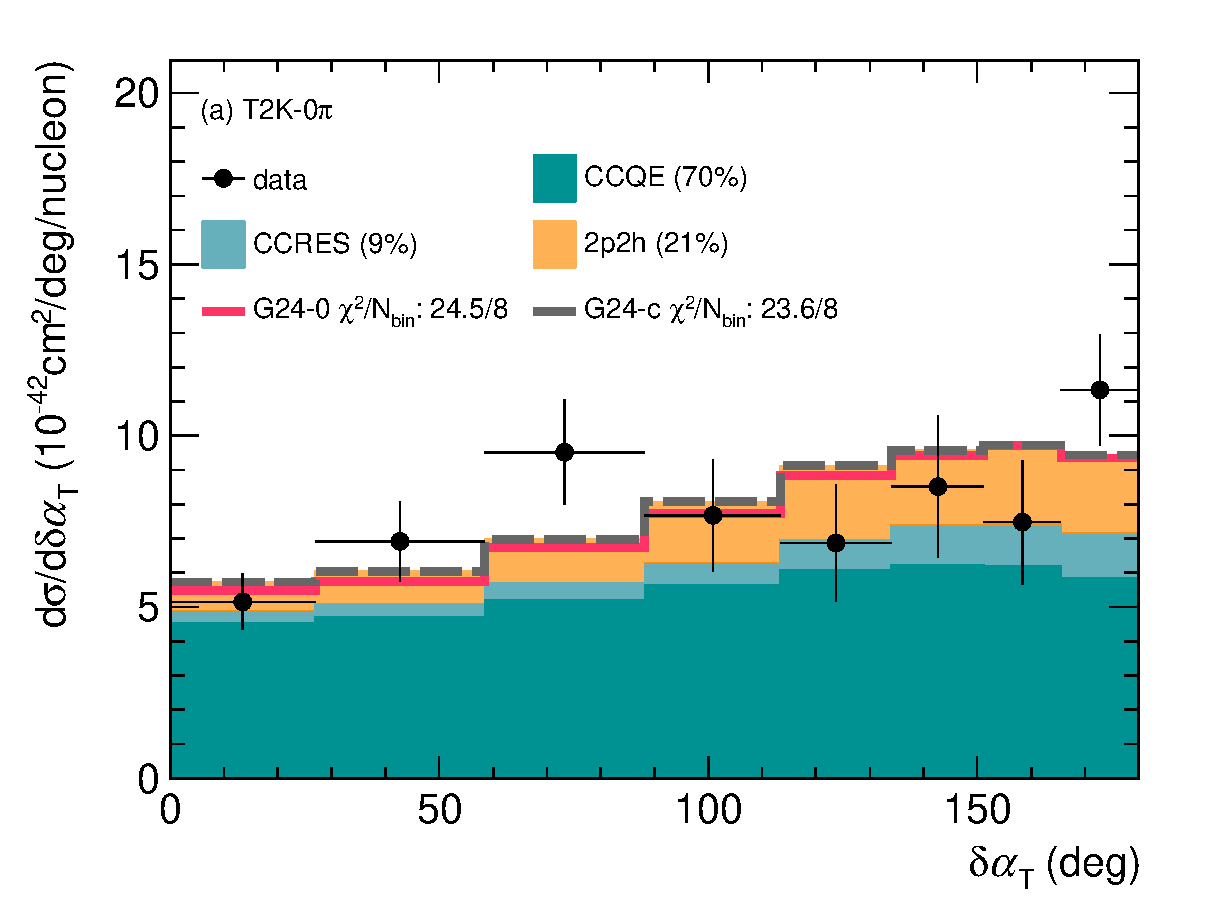
\includegraphics[width=\dbfigwid\textwidth]{figures/tuning/0026-t2k_0pi_dalphat_reac_decomp_covfix.eps}
    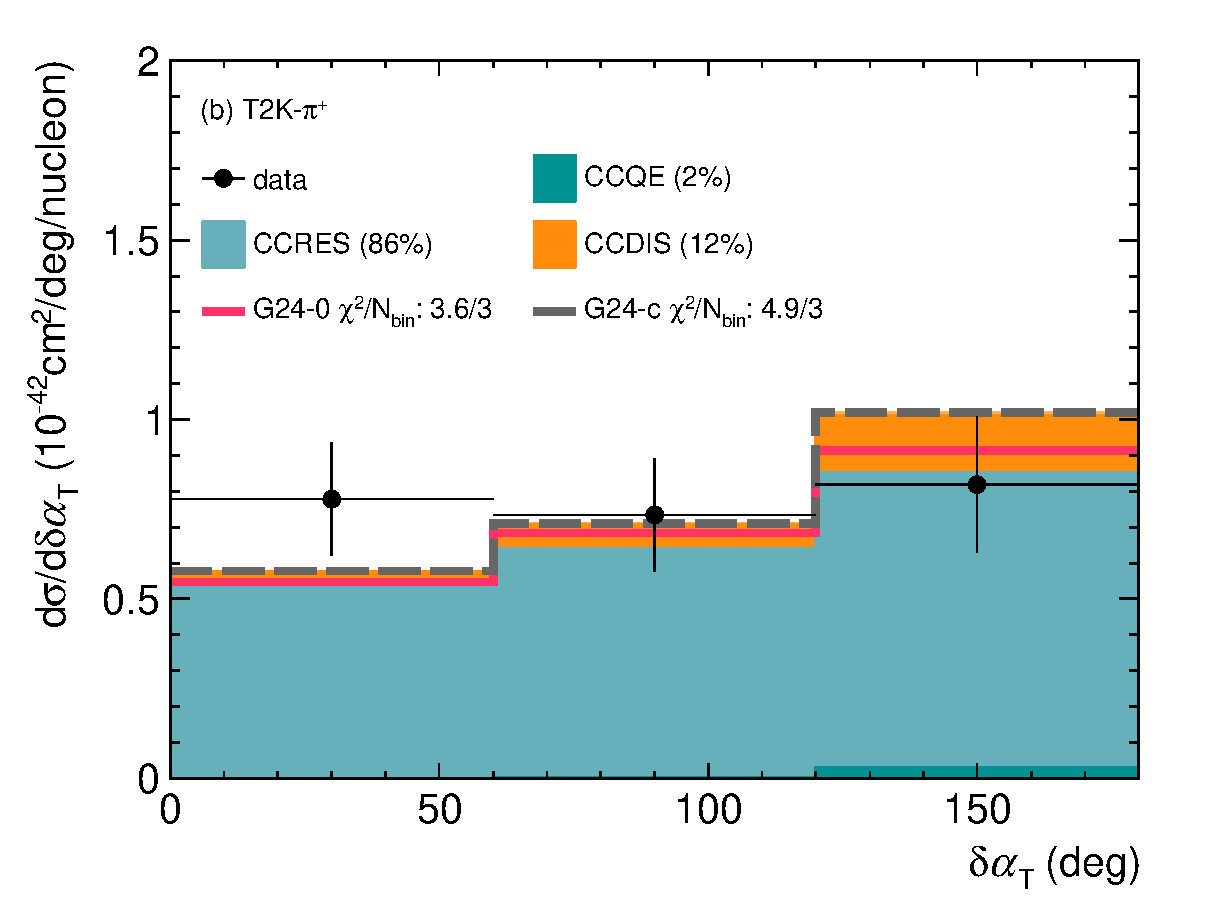
\includegraphics[width=\dbfigwid\textwidth]{figures/tuning/0026-t2k_pip_dalphat_reac_decomp_covfix.eps}
    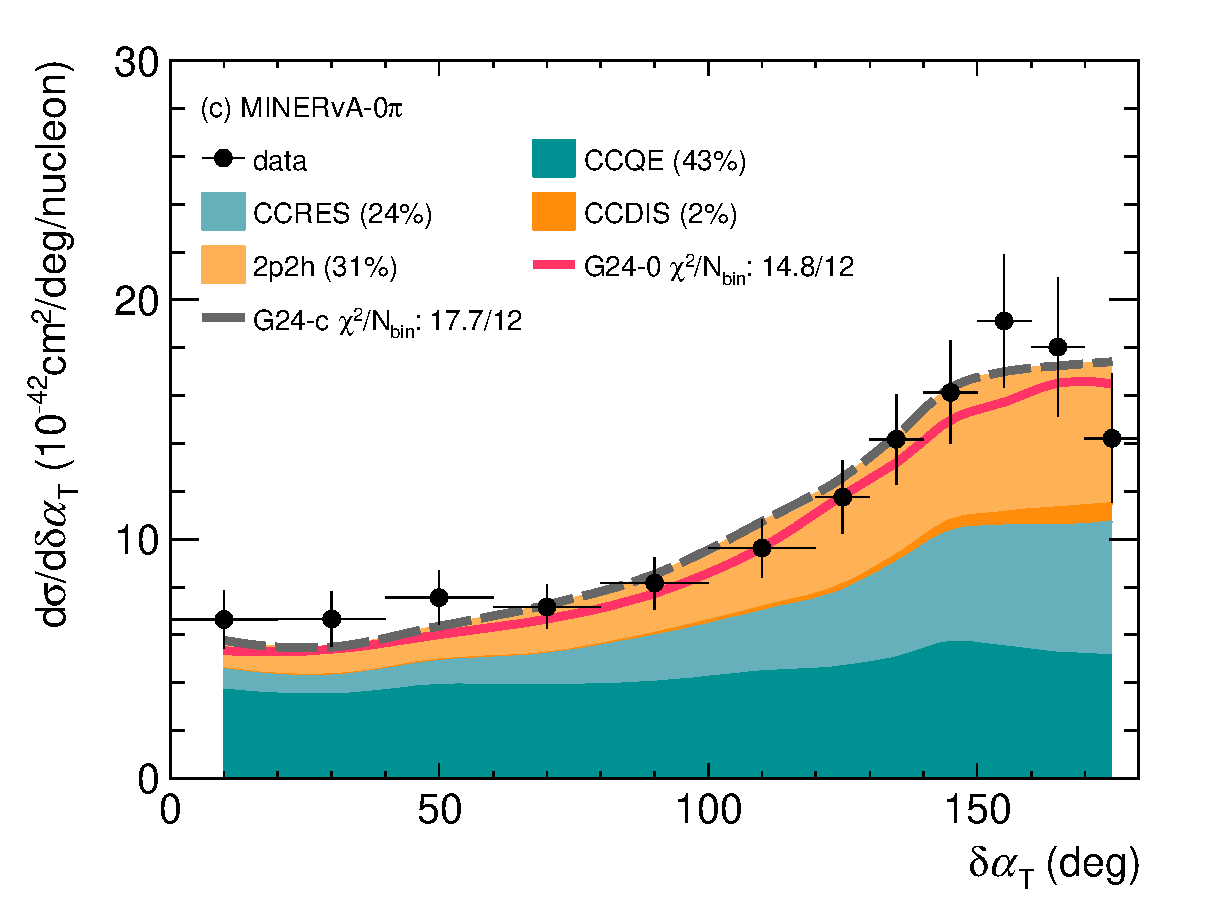
\includegraphics[width=\dbfigwid\textwidth]{figures/tuning/0026-min_0pi_dalphat_reac_decomp_covfix.eps}
    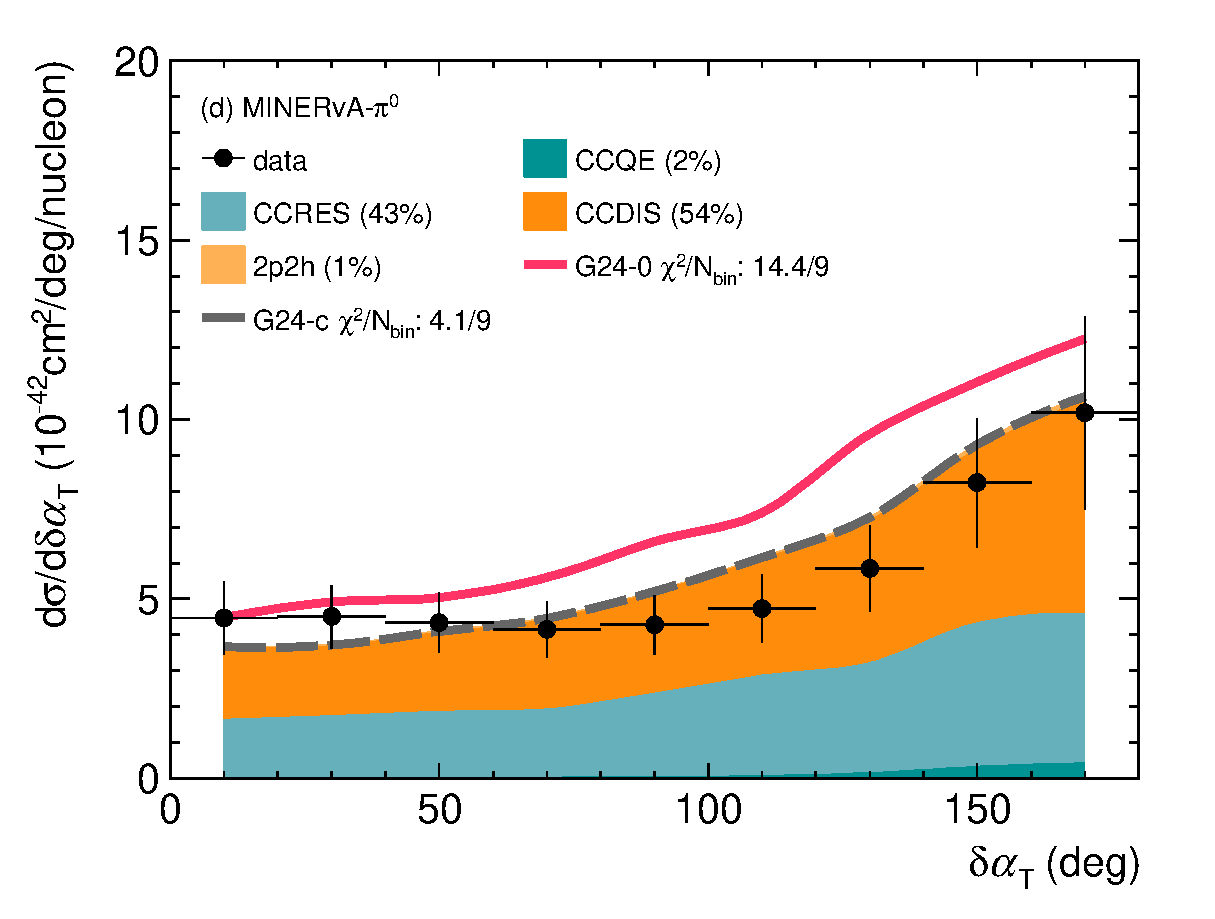
\includegraphics[width=\dbfigwid\textwidth]{figures/tuning/0026-min_pi0_dalphat_reac_decomp_covfix.eps}
    \caption{\label{fig:g24-c-dat-reac} 
    Similar to Fig.~\ref{fig:g24-0-dat-reac} but with \gC.  The \gZero prediction is also plotted for comparison. 
    } 

    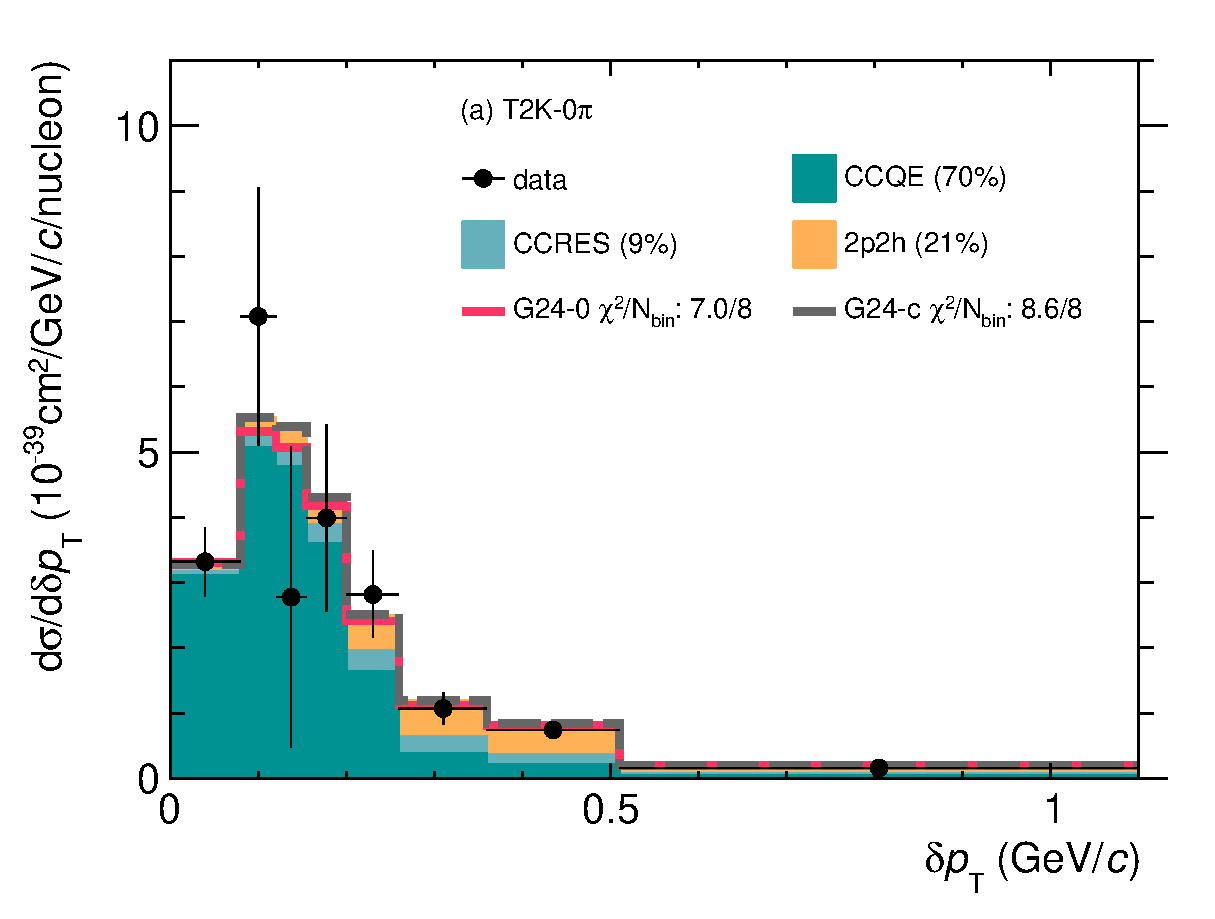
\includegraphics[width=\dbfigwid\textwidth]{figures/tuning/0026-t2k_0pi_dpt_reac_decomp_covfix.eps}
    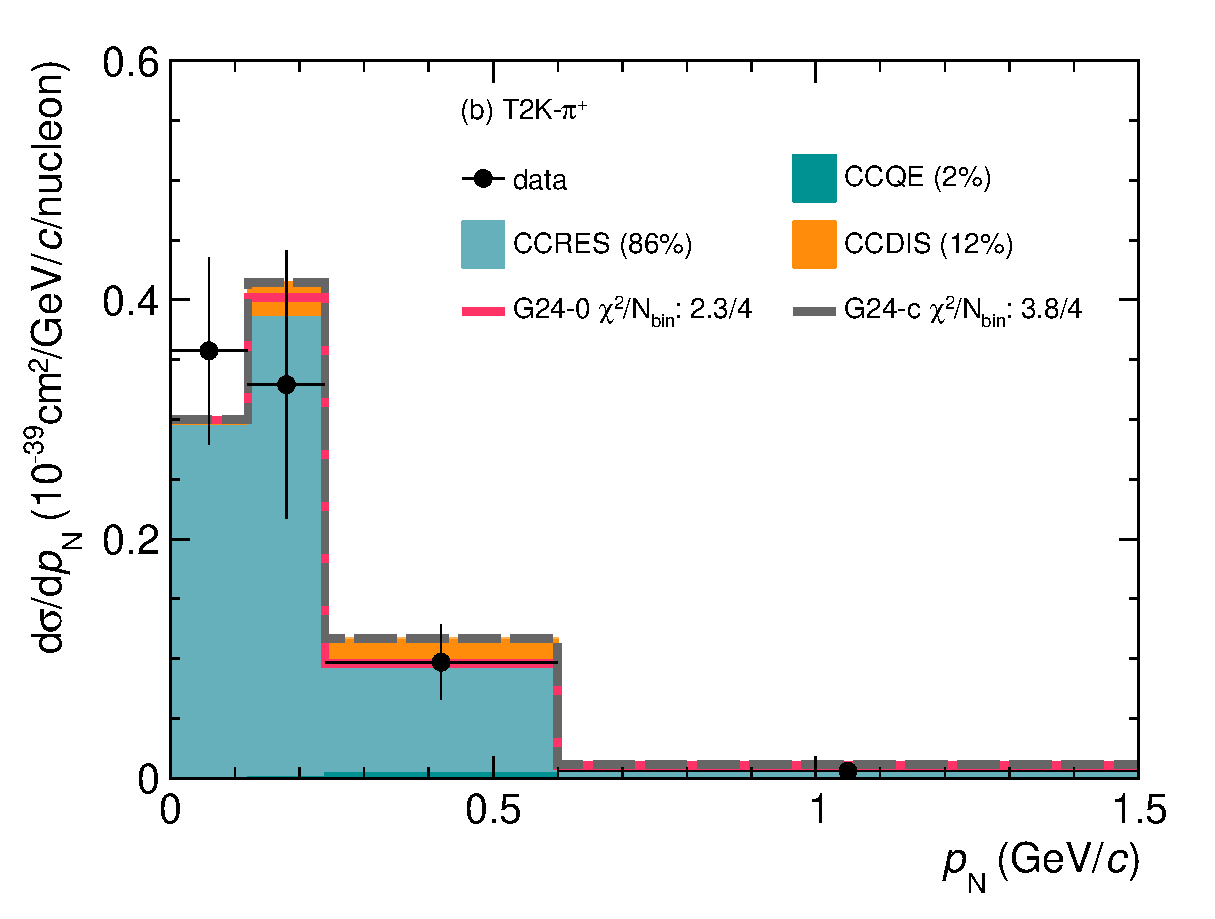
\includegraphics[width=\dbfigwid\textwidth]{figures/tuning/0026-t2k_pip_pn_reac_decomp_covfix.eps}	
    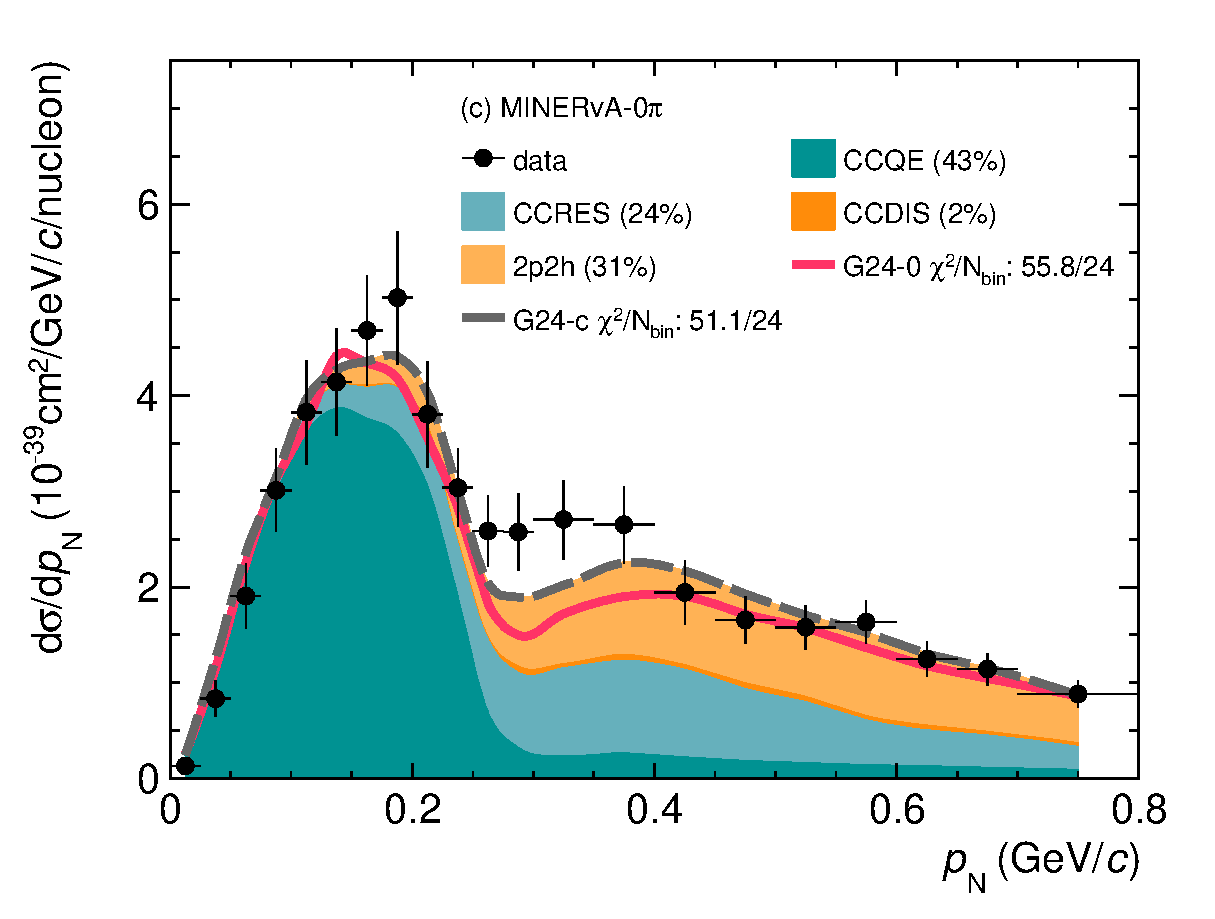
\includegraphics[width=\dbfigwid\textwidth]{figures/tuning/0026-min_0pi_pn_reac_decomp_covfix.eps}
    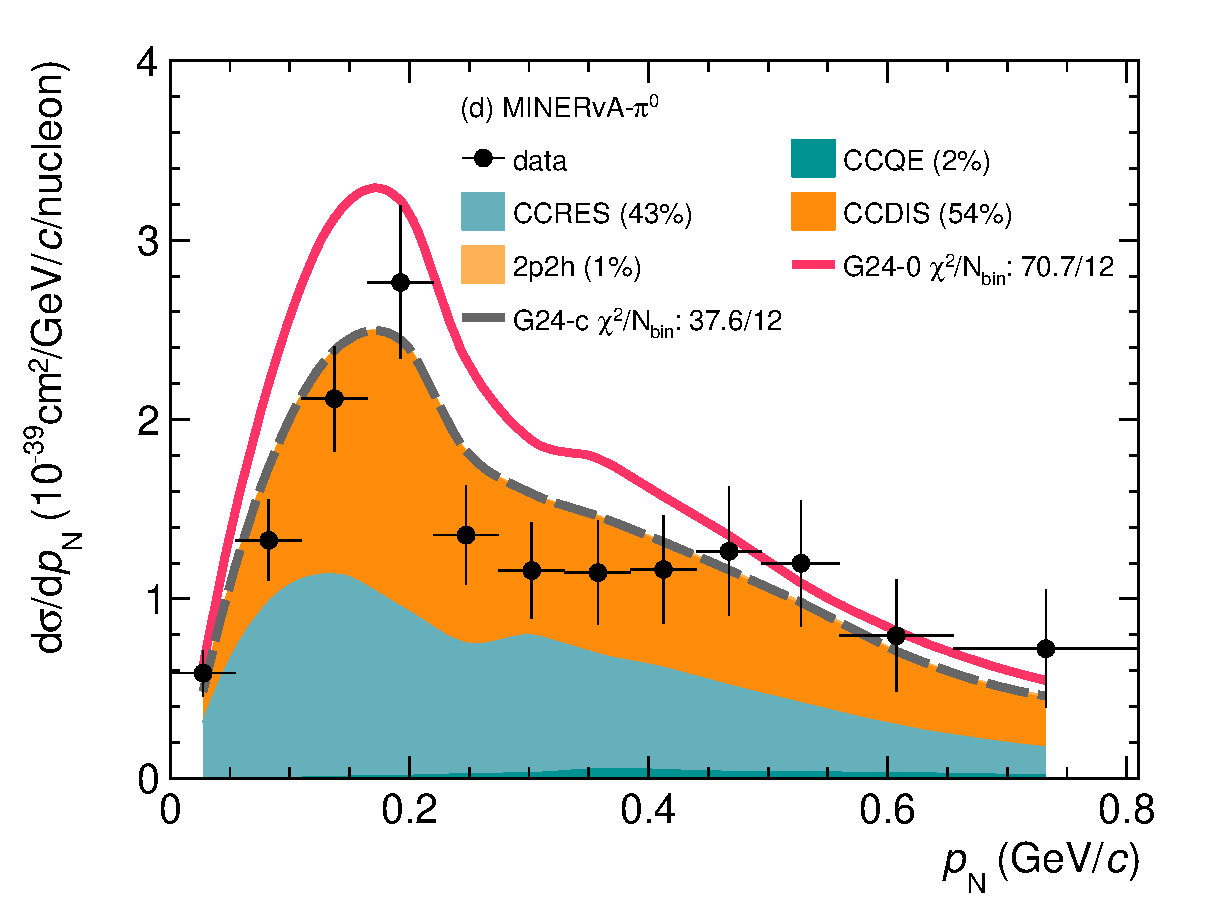
\includegraphics[width=\dbfigwid\textwidth]{figures/tuning/0026-min_pi0_pn_reac_decomp_covfix.eps}
    \caption{\label{fig:g24-c-pn-reac}  
    Similar to Fig.~\ref{fig:g24-c-dat-reac} but for the $\pn$ (\ttkpip, \minzpi and \minpiz) and $\dpt$ (\ttkzpi) measurements. 
    } 
\end{figure*}

Given the intricate correlations among model parameters, determining which ones are most sensitive to the data proves challenging. Considerable correlation and anti-correlation are observed between different FSI fates for the same particle, e.g. $\cpiabs$ and $\pipiprod$, as shown in Figs.~\ref{fig:comb_26_cor_allpar} and~\ref{fig:comb_26_cor_redpar}. 
Our tuning began with the \allpar\ parameter set, achieving the best result with \texttt{Combi-13}, which is denoted as \cbAllPar\ in Table~\ref{tab:data-sets} (cf. Fig.~\ref{fig:allchi} for the $\chi^2$ distribution of all combinations).
Observations showed that for most combinations, certain parameters remained close to their default values, within $1$ $\sigma$ of the imposed priors, such as $\pipiprod$ since none of the data sets has a significant contribution from PIPD of pions---Removing these parameters from the tuning process does not significantly affect the outcome.
Therefore, we then constructed a reduced set comprising only $\srcfr$, $\pizmfp$, $\picex$, $\ncex$, $\nabs$, and $\npiprod$ (denoted as \redpar\ in Table~\ref{tab:hALFG-para}) and ran the tuning on the 26 combinations with it. Note that the parameters most correlated with $\picex$ and $\pizmfp$ are not present in \redpar\. The \redpar\ tuning proved more stable, with nearly all combinations showing a more negative $\chi^2$ change than the \allpar\ tuning, as shown in Fig.~\ref{fig:allchi}. Moreover, the single-observable (\texttt{Combi-}1 to 5), single-measurement (\texttt{Combi-}6 to 9), single-experiment (\texttt{Combi-}10 and 11), and single-topology (\texttt{Combi-}12 and 13) combinations all systematically yielded no or limited overall (tuned plus validation) improvement post-tuning. The best tuning then occurred with \texttt{Combi-26} (\cbRedPar\ in Table~\ref{tab:data-sets}), that is, all TKI variables excluding $\dphit$ and $\dpt$ (unless no $\pn$ is available)---$\dat$, $\pn$ (or $\dpt$ if $\pn$ is unavailable), and $\dptt$---from pionless and pion-production measurements in both T2K and MINERvA. 

Table~\ref{tab:restunes} summarizes the primary results of our tuning process. The tuned \redpar\, \restunefull (\gC), is derived from the observable set \cbRedPar\, and the tuned \allpar\, $\alttune$~(\gT), is from \cbAllPar\. The upper part of Table~\ref{tab:restunes} contains the parameter values. 
For the  \gC\ tune, changes to the \sfcfg\ model were moderately sized ($\srcfr$ decreases from $0.12$ to $0.09$), while in the hA model, $\pizmfp$ and $\picex$ are highly suppressed and the nucleon FSI has larger CEX and PIPD and lower ABS.  The tune \gT\ differs most significantly from \gC\ in $\pizmfp$ and $\picex$. The table's lower section illustrates $\chi^2$ improvements for selected observables and their corresponding validation sets. Crucially, tuning should not reduce the accuracy of validation set descriptions. Overall, \gC\ has a more substantial reduction in the total $\chi^2$. In the following, we will discuss the two tunes.

\begin{table}[!htb]
    \centering
    \begin{tabular}{cccc}
    \hline
    \hline
    Parameter              & Nominal (\gZero) &  \redpar (\gC)     & \allpar (\gT)   \\
    \hline
    \multicolumn{4}{c}{\sfcfg} \\
    \hline
    $\srcfr$   & 0.12 & 0.09 $\pm$ 0.08         & 0.17  $\pm$ 0.10       \\
    $\nurmec$  & 0.01 & 0.01                    & 0.06 $\pm$ 0.000004     \\
    \hline
    \multicolumn{4}{c}{hA} \\
    \hline
    $\cpimfp$  & $1.0\pm0.2$ & 1.0                      & 1.21   $\pm$ 0.15         \\
    $\pizmfp$  & $1.0\pm0.2$ & 0.34 $\pm$ 0.11          & 0.91   $\pm$ 0.000004     \\
    $\nmfp$    & $1.0\pm0.2$& 1.0                       & 0.89   $\pm$ 0.000382     \\
    \hline
    $\picex$   & $1.0\pm0.5$ & 0.27 $\pm$ 0.28          & 0.86   $\pm$ 0.000056      \\
    $\ncex$    & $1.0\pm0.4$ & 1.39 $\pm$ 0.33          & 0.92  $\pm$ 0.001178       \\
    \hline
    $\piinel$  & $1.0\pm0.4$ & 1.0                      & 0.90   $\pm$ 0.00008       \\
    $\ninel$   & $1.0\pm0.4$ & 1.0                     & 0.92   $\pm$ 0.001218       \\
    \hline
    $\cpiabs$  & $1.0\pm0.2$ & 1.0                      & 1.36   $\pm$ 0.38          \\
    $\pizabs$  & $1.0\pm0.2$ & 1.0                      & 0.92   $\pm$  0.000024     \\
    $\nabs$    & $1.0\pm0.2$ & 0.48 $\pm$ 0.33          & 1.02   $\pm$ 0.413668      \\
    \hline
    $\pipiprod$& $1.0\pm0.2$ & 1.0                      & 1.11   $\pm$ 0.342484       \\
    $\npiprod$ & $1.0\pm0.2$ & 1.90 $\pm$ 0.71          & 1.12   $\pm$ 0.57198        \\ 
    \hline
    \hline
    \multicolumn{4}{c}{$\chi^2$ \textrm{for} \texttt{combi}} \\
    \hline
    \texttt{untuned}         & & 231.75         & 129.61        \\
    \texttt{tuned}           & & 168.67         & 131.46        \\
    \texttt{diff}            & & -63.08         & 1.85         \\
    \hline
    \multicolumn{4}{c}{$\chi^2$ \textrm{for} \texttt{vald}} \\
    \hline
    \texttt{untuned}    & & 229.5          & 331.64        \\
    \texttt{tuned}            & & 232.3    & 304.4         \\
    \texttt{diff}       & & 2.8          & -27.24        \\
    \hline
    \multicolumn{4}{c}{$\chi^2$ \textrm{for} \texttt{combi+vald}} \\
    \hline
    \texttt{untuned}    & &  461.25          &  461.25        \\
    \texttt{tuned}          &  & 400.97 & 435.86        \\
    \texttt{diff} & & -60.28         & -25.39  \\     
    \hline
    \hline
\end{tabular}
\caption{\label{tab:restunes}
	Parameters in \gZero, \gC, and \gT. Those without errors are not tuned. Lower section: \texttt{combi} indicates that the following $\chi^2$ sums are calculated for the tuned measurements (i.e. \cbRedPar (98 bins) and \cbAllPar (46 bins) for \gC and \gT, respectively), while \texttt{vald} indicates that the respective validation sets are used; \texttt{untuned} means that the $\chi^2$ calculation uses the nominal values of the parameters, while \texttt{tuned} denotes the tuned ones. \texttt{diff} displays the improvement achieved by the respective tuning.  
}
\end{table}


\subsection{Reduced tune: \gC}

To assess the tune's quality, we plot predictions using \gC\ for $\dat$ and $\pn$ in Figs.~\ref{fig:g24-c-dat-reac} and~\ref{fig:g24-c-pn-reac},  respectively. For \ttkzpi\, \ttkpip\ and \minzpi\, the new $\chi^2$ values are comparable to those obtained with \gZero, changing less than the number of bins. For \minpiz\, \gC\ is distinctly better than \gZero, thereby demonstrating the possibility of simultaneous good descriptions of both pionless and pion production samples with constrained parameters from cross-topology TKI tuning. Note that in the region of $\pn\sim0.3~\gevc$, the model deficit previously reported in Ref.~\cite{MINERvA:2018hba} (and also shown in Fig.~\ref{fig:g24-0-pn-reac}c) persists even after the fit. The physical origin of this deficit might be attributed to the strength of the 2p2h contribution~\cite{MINERvA:2018hba}, but it is still a topic of significant discussion within the community.

Examining individual datasets closely helps to understand the origin of the improvement. The decomposition of the cross section for $\dat$ according to the FSI fates of the $\piz$ is presented in Fig.~\ref{fig:CEX-minpiz-dat-pi0}. The hA model rescatters primary interaction products only once, and records this event with a rescattering code for these particles. The rescattered products, which are the final outputs, are stored as daughters of the primary interaction products. Hence, the FSI fate that produces the final products can be checked by the rescattering code of their first parent. More specifically, we loop through all final-state particles to look for the leading $\piz$ and check the rescattering code of its first parent. 

\begin{figure}[!htb] 	
    \centering 		
    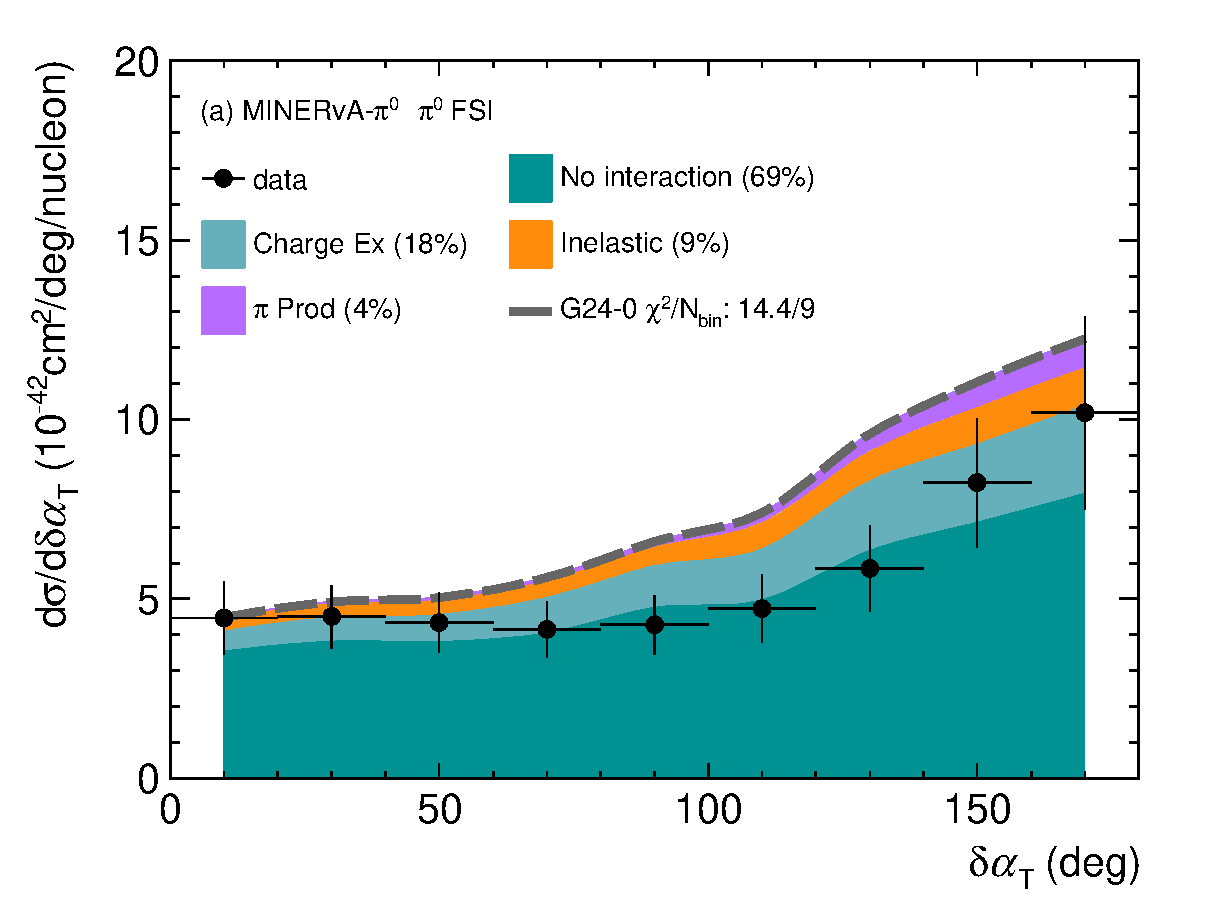
\includegraphics[width=\dbfigwid\textwidth]{figures/tuning/0000-min_pi0_dalphat_pi0_decomp_cex.eps}
    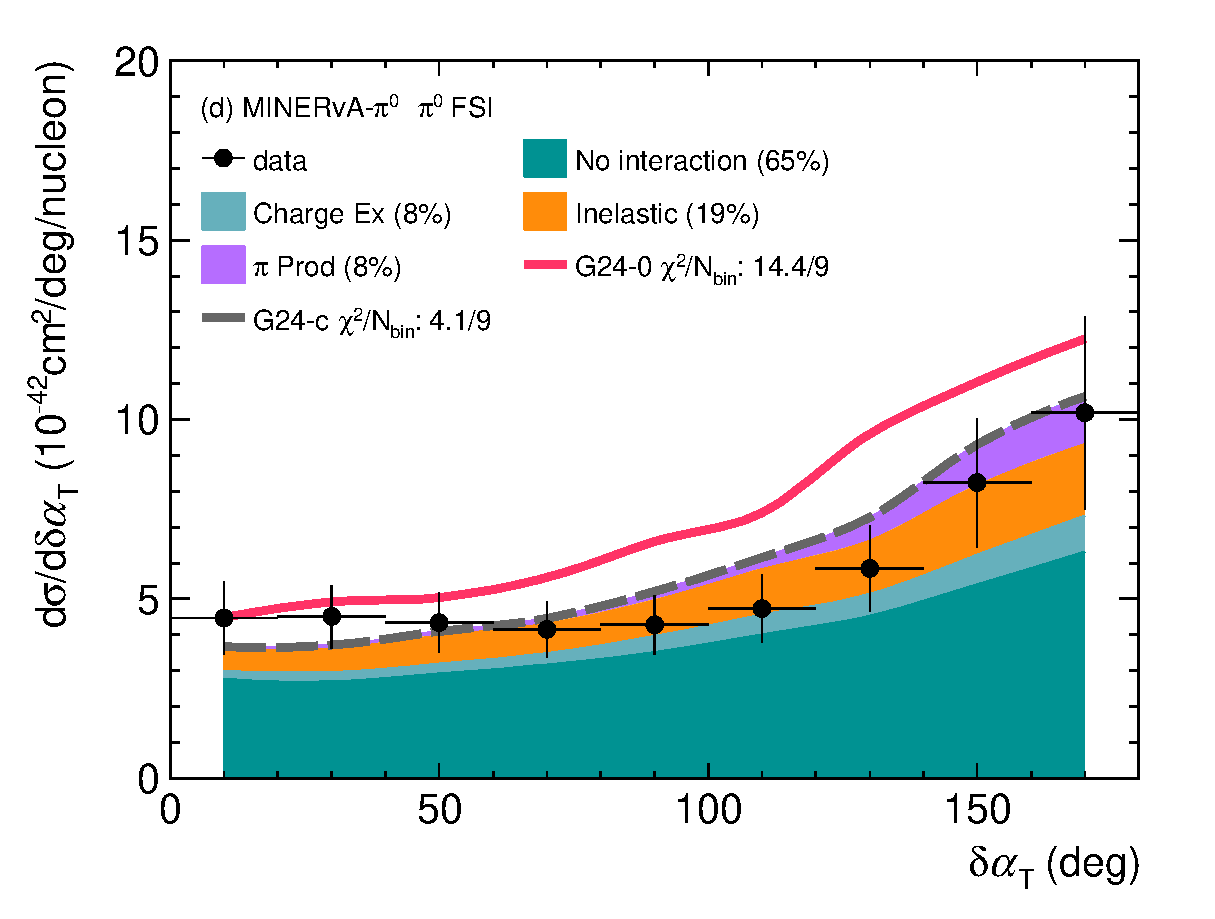
\includegraphics[width=\dbfigwid\textwidth]{figures/tuning/0026-min_pi0_dalphat_pi0_decomp_covfix.eps}	
    \caption{\label{fig:CEX-minpiz-dat-pi0} \minpiz\ $\dat$ measurement compared to \genie predictions decomposed in $\piz$ FSI fates with (a) \gZero\ and (b) \gC.} 
\end{figure}

In \minpiz\, the number of $\piz$s undergoing no FSI (``No Interaction'', as shown in the figures) is adjustable via the $\pizmfp$ parameter. A decrease in $\pizmfp$ reduces the size of the ``No Interaction'' events,  as is shown in Fig.~\ref{fig:CEX-minpiz-dat-pi0}b when compared to Fig.~\ref{fig:CEX-minpiz-dat-pi0}a. Meanwhile, an increase in $\piz$ rescattering only manifests in pionless measurements through ABS. There is indeed an increase of ABS for $\piz$ in \ttkzpi\ and \minzpi\, but the fraction is small to begin with, so the impact is small. The increase of $\piz$ rescattering can increase \ttkpip\ via CEX as discussed below. However, due to the significant suppression of CEX, its impact on \ttkpip\ is also minimal (for detailed breakdown, see Figs.~\ref{fig:g24-0-dat-pi0}-\ref{fig:g24-c-pn-pi0} in Appendix~\ref{sec:appfate}). 

As shown in Fig.~\ref{fig:CEX-minpiz-dat-pi0}a, the \minpiz\ prediction from the nominal tune has considerable contributions from CEX controlled by $\picex$. It does not impact \ttkzpi\ and \minzpi\ as CEX only changes the pion type without removing them. Hence, events with pions in the final state would be rejected in these two data sets regardless of the pion charge. In principle, CEX will also migrate events between the signal and background definitions for \ttkpip\ when a $\piz$ is converted to a $\pip$ and vice verse. However, \ttkpip\ does not have a considerable CEX fraction to begin with, so changing CEX will have a minimal impact on its prediction. Hence, this is one of the most effective paths to decrease the \minpiz\ cross section prediction without affecting other measurements, and indeed the $\picex$ is heavily suppressed as shown in Table~\ref{tab:restunes} and illustrated in Fig.~\ref{fig:CEX-minpiz-dat-pi0}b compared to Fig.~\ref{fig:CEX-minpiz-dat-pi0}a. However, due to the intricate correlation between the FSI fates in the hA implementation discussed in Sec.~\ref{sec:tuning-para-choice}, although $\piinel$ and $\pipiprod$ are not modified explicitly, a considerable increase is observed in both INEL and PIPD for \minpiz. 

Suppressing both ``No Interaction'' and CEX for $\piz$ adjusts the \minpiz\ prediction to the appropriate magnitude with small impacts on other data sets.  The effects of the other parameter changes are more transparent in the comparison of the $\pn$ distribution of \minpiz\ between Figs.~\ref{fig:minpiz-pn-pr}a and~\ref{fig:minpiz-pn-pr}b. A relatively large increase in $\ncex$ and $\npiprod$ moves events away from the Fermi motion peak at $\pn\leq0.25~\textrm{GeV}/c$; the same effect can be achieved by an increased $\srcfr$. 

Another impact of the larger $\npiprod$ manifests in the appearance of 2p2h ($1\%$) and CCQE ($2\%$) in the \minpiz\ cross section, as shown in Fig.~\ref{fig:g24-c-pn-reac}d. These neutrino-nucleon interactions do not produce pions, but the product nucleons can produce pions via re-scattering in the nucleus, leading to a contribution to topologies with pions in the final states. However, such contribution remains small.

\begin{figure}[!htb] 	
    \centering 		
    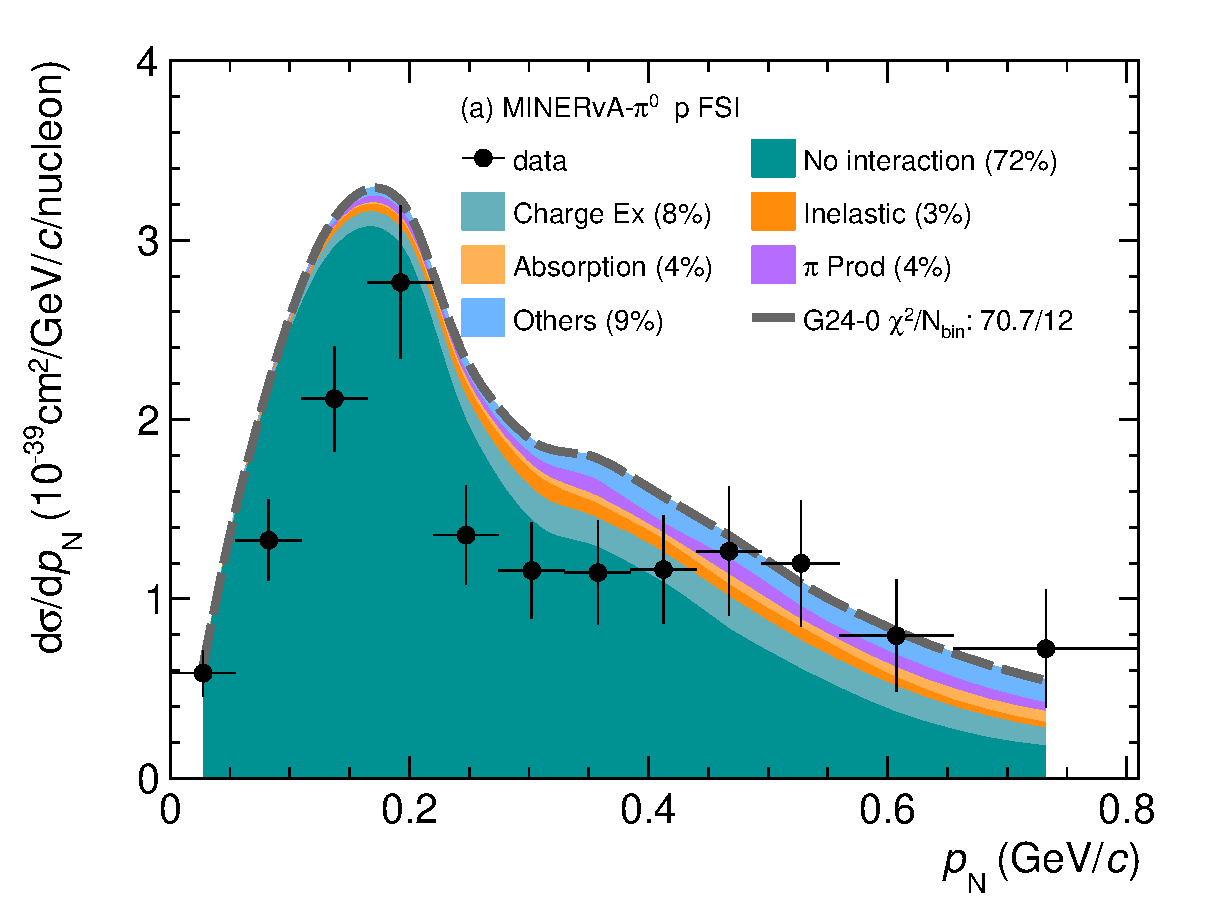
\includegraphics[width=\dbfigwid\textwidth]{figures/tuning/0000-min_pi0_pn_pr_decomp_cex.eps}
    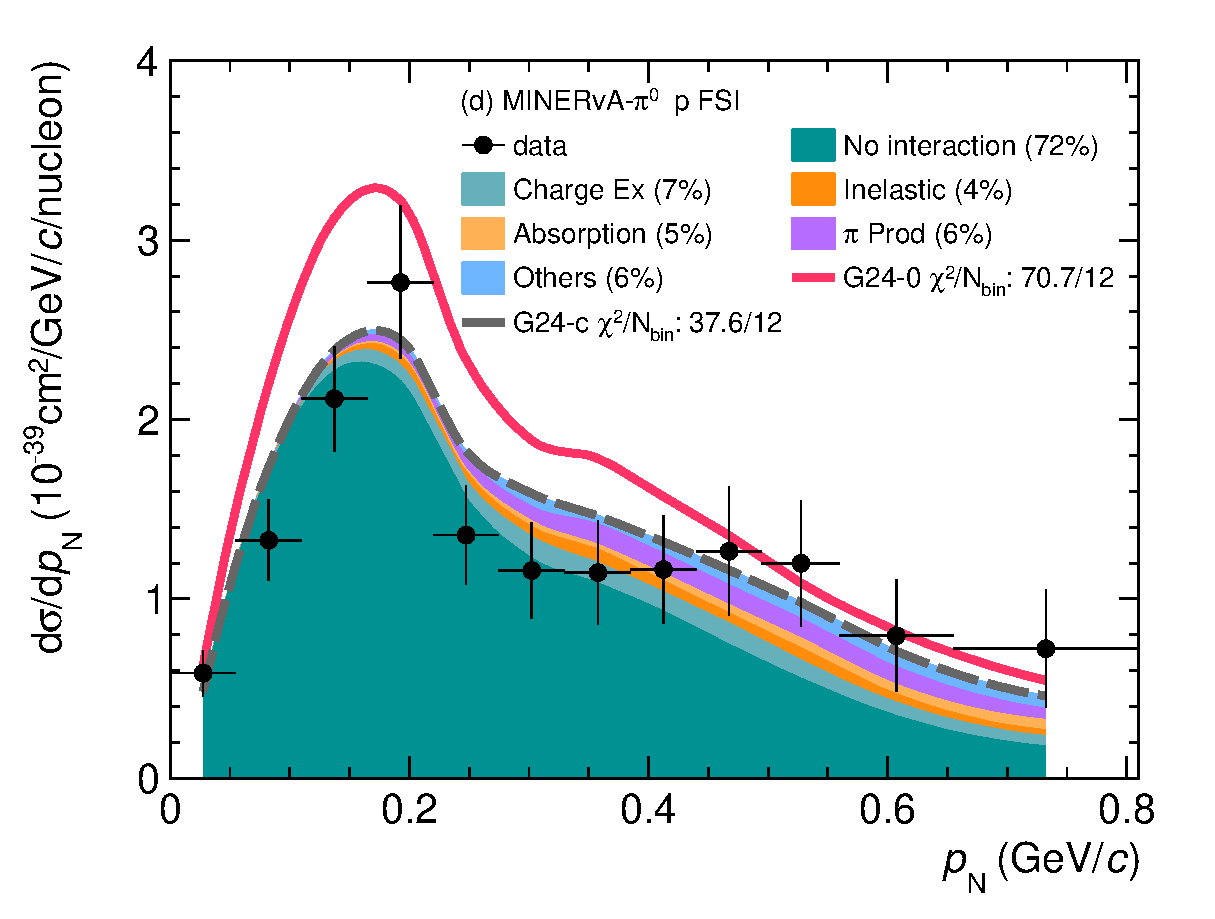
\includegraphics[width=\dbfigwid\textwidth]{figures/tuning/0026-min_pi0_pn_pr_decomp_covfix.eps}	
    \caption{\label{fig:minpiz-pn-pr} Similar to Fig.~\ref{fig:CEX-minpiz-dat-pi0} but for $\pn$ with proton FSI fate decomposition. Note that the ``Absorption'' of the proton is referring to the absorption of the $\pip$ from the decay of $\deltapp$, which could lead to emission of nucleons as discussed in Sec.~\ref{sec:tuning-para-choice}.     
    } 
\end{figure}

Although the interaction models, e.g. 2p2h, are not directly tuned, the respective fractions have undergone small changes in Fig.~\ref{fig:g24-c-dat-reac} and Fig.~\ref{fig:g24-c-pn-reac}, compared to Fig.~\ref{fig:g24-0-dat-reac} and Fig.~\ref{fig:g24-0-pn-reac}. 
This is a result of the increased $\srcfr$ which leads to more events with higher initial nucleon momenta such that interactions requiring higher initial state energy, such as RES and DIS, will be more frequent. 
This is reflected by the increase in the ratios of these interactions: For example, RES increases from $19\%$ (Fig.~\ref{fig:g24-0-pn-reac}c) to $24\%$ (Fig.~\ref{fig:g24-c-pn-reac}c) for \minzpi. 
Hence, the other interactions, although not directly tuned, will experience a decrease in the fraction of total cross section: For example, 2p2h drops from $31\%$ (Fig.~\ref{fig:g24-0-pn-reac}c) to $30\%$ (Fig.~\ref{fig:g24-c-pn-reac}c) for \minzpi.



\subsection{Alternative tune: \gT}

A considerably smaller improvement is achieved by the intermediate tune, \gT, illustrated in Fig.~\ref{fig:minpiz-alttune}. Instead of significantly increasing proton PIPD to elevate the $\pn$ tail, this tune notably enhances $\srcfr$---more-energetic nucleons are present and therefore the RES $\pn$ peak is shifted to the right in Fig.~\ref{fig:minpiz-alttune}a with respect to Fig.~\ref{fig:g24-c-pn-reac}d. Rather than suppressing $\picex$ and $\pizmfp$ heavily (cf. Fig.~\ref{fig:g24-c-pn-pi0}d in Appendix~\ref{sec:appfate}), this tune slightly decreases them. Overall, this leads to a moderate reduction of $25.39$ in $\chi^2$ (Table~\ref{tab:restunes}), as well as a relatively improved data-MC agreement across all data sets. 

\begin{figure}[!htb] 	
    \centering 		
    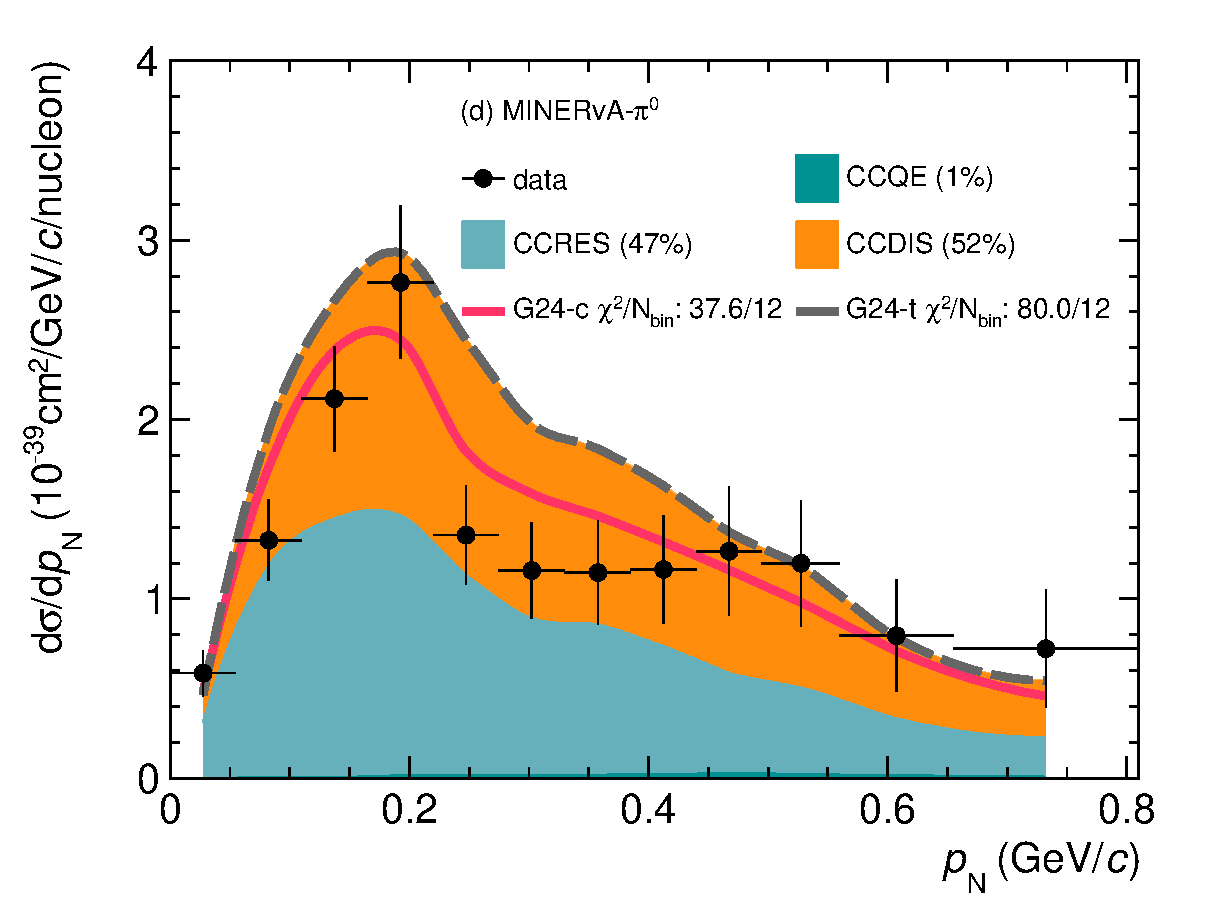
\includegraphics[width=\trfigwid\textwidth]{figures/tuning/0013-min_pi0_pn_reac_decomp.eps}
    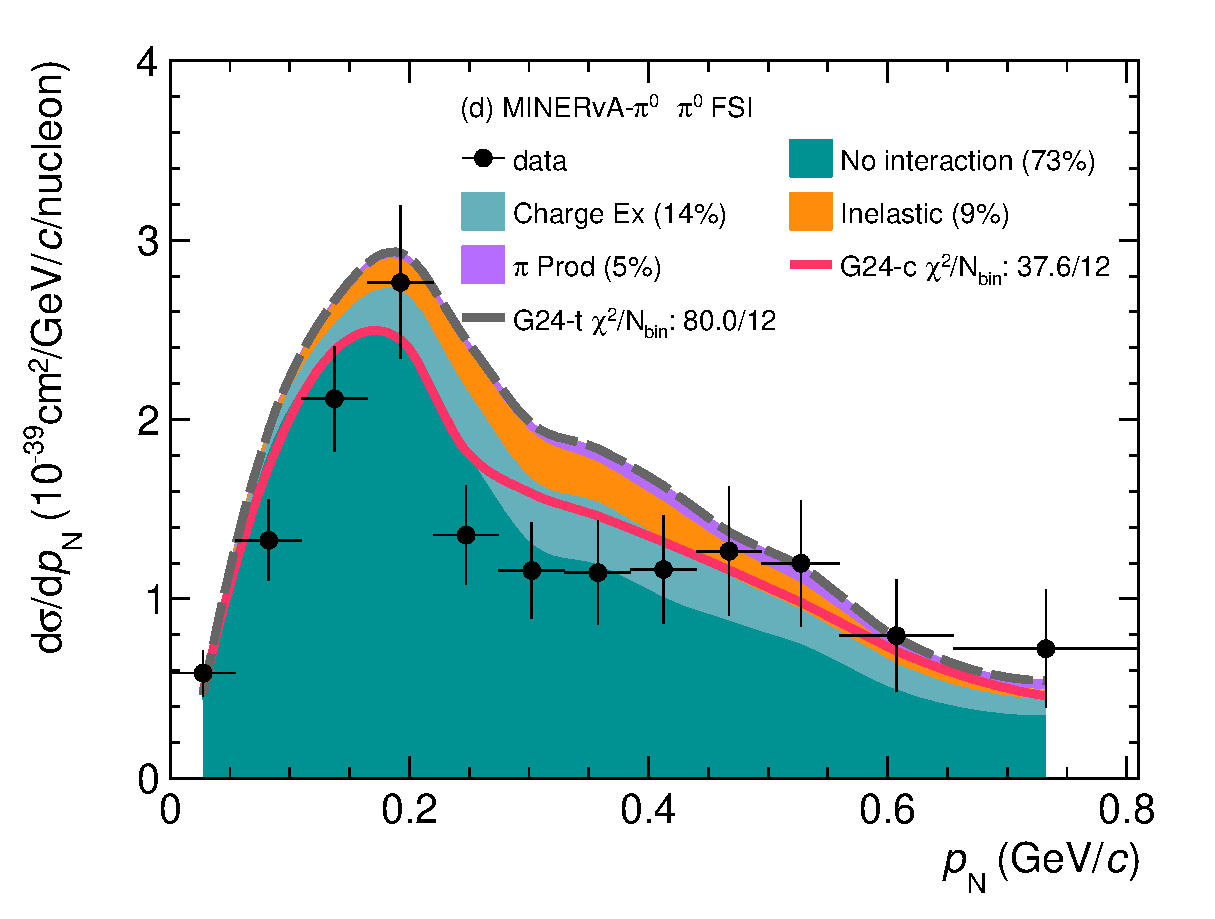
\includegraphics[width=\trfigwid\textwidth]{figures/tuning/0013-min_pi0_pn_pi0_decomp.eps}
    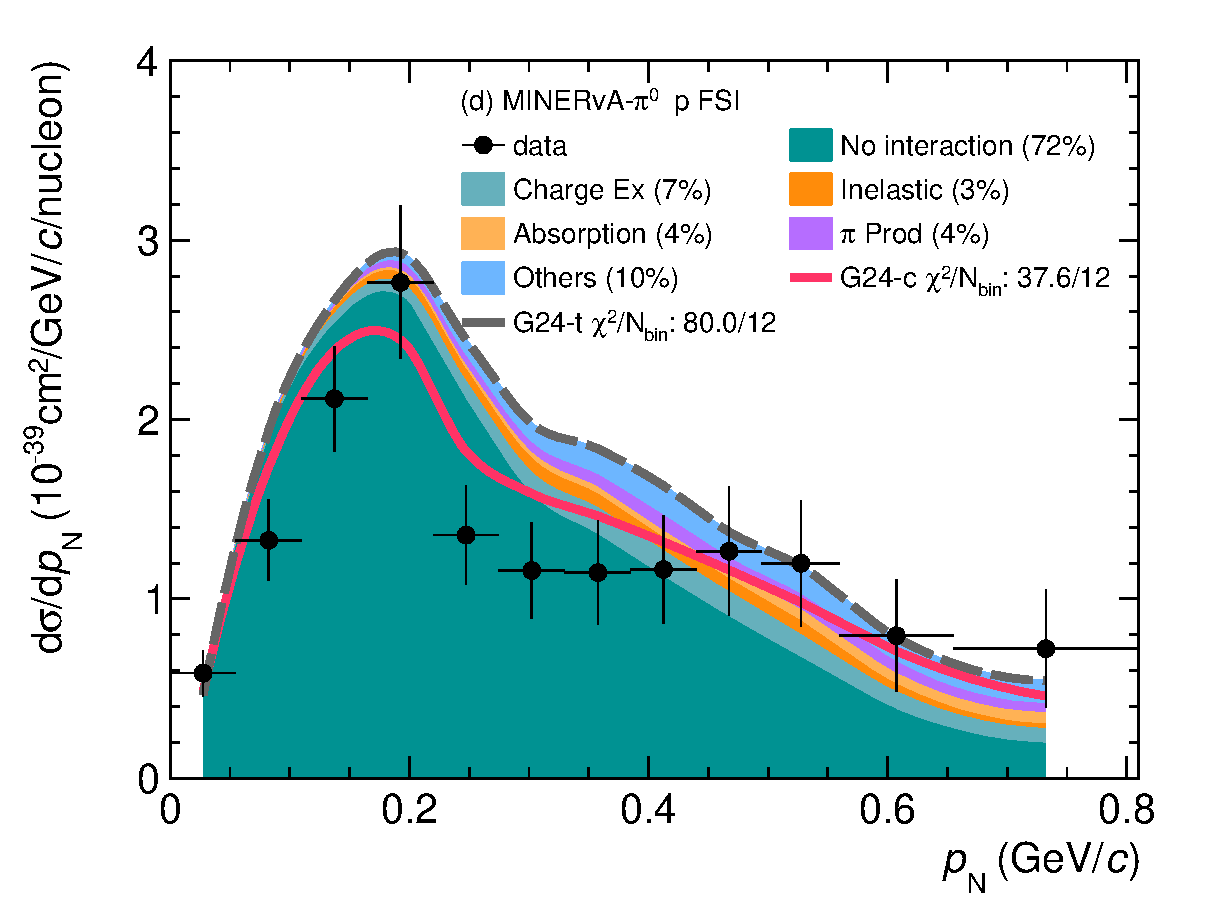
\includegraphics[width=\trfigwid\textwidth]{figures/tuning/0013-min_pi0_pn_pr_decomp.eps}
    \caption{\label{fig:minpiz-alttune} \minpiz $\pn$ measurement compared to \genie predictions decomposed in  (a) $\nu$-N interaction, (b) $\piz$ FSI, and (c) proton FSI for the alternative tune, \gT.} 
\end{figure}


\subsection{Discussion}
For both \gC\ and \gT\ the fit results suggest extreme values, but the effect of the parameter change is less effective than the change in the parameter suggests. 
For the individual FSI fate cross section, due to the re-normalization step after scaling, the effective change for one particular fate is smaller than the scaling parameter magnitude as explained in Sec.~\ref{sec:tuning-para-choice}. 
As for the total FSI cross sections, only that of $\piz$ is changed. The total $\piz$-C scattering cross section for pion kinetic energy is plotted in Fig.~\ref{fig:pizmfp_change} to assess the overall impact. 
The shape remains similar and consistent with Fig. 2.23 ($\pip$-C reactions) in Ref.~\cite{Andreopoulos:2015wxa} while the peak magnitude increases from $380$ to $489$ mb, a $29\%$ increase, considerably less than the scaling factor, $\pizmfp=0.34$, seemingly suggests. 
Moreover, the default $\piz$ parameter values are calculated from charged pion data assuming isospin symmetry rather than extracted directly from experimental data. 
Hence, this modification does not violate any existing agreement with hadron scattering data.
\begin{figure}[!htb] 	
    \centering 		
    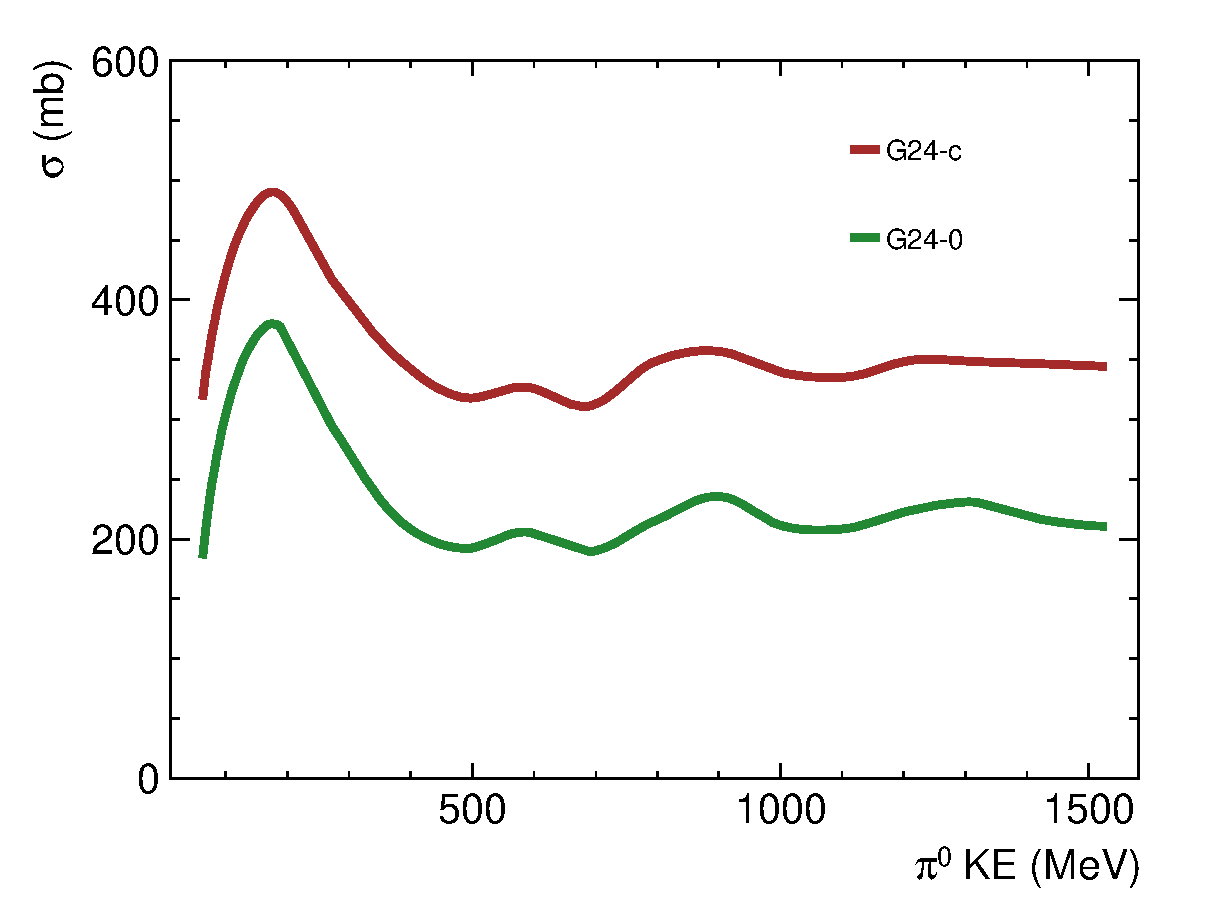
\includegraphics[width=\sgfigwid\textwidth]{figures/tuning/pi0mfp_change_covfix.eps}
    \caption{\label{fig:pizmfp_change} Change in MC prediction for $\piz$ cross section between \gZero and \gC . } 
\end{figure}
In addition, agreement of this tune with most of the non-TKI neutrino datasets available is unchanged before and after the tune,  thereby demonstrating the physicality of the tune.

Exclusive electron scattering data is better suited to constrain FSI models.
Regrettably, most electron scattering data to date is inclusive~\cite{electronsforneutrinos:2020tbf} and it is not well suited for the tuning of FSI. 
The ``Electrons for Neutrinos'' (e4nu) collaboration exploits data from the CLAS6 spectrometer to measure exclusive final states, such as a $1\textrm{p}0\pi$ cross-section measurement on carbon as a function of TKI variables~\cite{CLAS:2021neh}. But for electron-scattering pion production, 
currently, the \genie predictions over-predict data due to the lack of tuning of the \genie models on free nucleon data.
Such big uncertainties in the pion production model mask possible nuclear model or FSI dependence.
In order to be sensitive to these effects, one need to first tune electron-scattering to free nucleon data. The current tuning study could be extended in the future when data from dedicated electro-pion production measurements are available. 

In conclusion, this tune is a valid and effective model that can be used as a starting point for an analysis. 
Further refinement will be available once more data will be included in the fit, including non-TKI observables and electron-scattering data.


\section{\label{sec:summary} Summary and outlook}
This work represents the first global tuning effort on TKI data. Our partial tune of the \sfcfg\ and hA models, $\restunefull$ (\gC), provides an effective theory to better describe both the neutrino-hydrocarbon pionless and pion production.
The largest change in the model is demanded by the \minpiz\ TKI measurement~\cite{MINERvA:2020anu} that was significantly overestimated in \genie. 
The improvement is crucial for future precision GeV neutrino experiments.  This tuning configuration has been integrated into the \texttt{master} branch of \genie and is slated for inclusion in the upcoming release.  

To develop an effective model, we focused on the most sensitive parameters, $\srcfr$, $\pizmfp$, $\picex$, $\ncex$, $\nabs$, and $\npiprod$, of the \sfcfg\ and hA models, reducing the total number of parameters from $14$ to $6$. The corresponding best combination of observables is $\dat$, $\pn$ (or $\dpt$ if no $\pn$ is available), and $\dptt$, from pionless and pion-production measurements in both T2K and MINERvA. 
In doing so, the pion production model is held fixed such that the tuned values of $\pizmfp$, $\picex$, $\nabs$, and $\npiprod$ depart from the established constraints from hadron measurements. 
A different pion production model might compensate part of these model tuning effects~\cite{Yan:2024kkg}. 
We also chose the hA FSI model for practical reasons. Its sequential treatment of MFP and rescattering should be considered as a numerical advantage (as was also pointed out in Ref.~\cite{GENIE:2022qrc}). Other more sophisticated models could be considered in future tunes.  With the existing four TKI measurements from T2K and MINERvA, we have also derived other effective tunes like $\alttune$ (\gT). The degeneracy can be resolved with additional data, particularly from argon-based measurements~\cite{MicroBooNE:2022emb, MicroBooNE:2023cmw, MicroBooNE:2023tzj, MicroBooNE:2023wzy, MicroBooNE:2024tmp, MicroBooNE:2015bmn} and e4nu data~\cite{CLAS:2021neh}.